\documentclass[11pt,b5paper]{book}

\usepackage{parskip}
\setlength{\parskip}{0.5em}
\setlength{\parindent}{1.5em}

\usepackage{longtable}
\usepackage{xcolor}
\usepackage{fontspec}
\setmainfont[
Path = fonts/,
UprightFont = TitilliumWeb-Regular.ttf,
BoldFont = TitilliumWeb-Bold.ttf,
ItalicFont = TitilliumWeb-Italic.ttf,
BoldItalicFont = TitilliumWeb-BoldItalic.ttf
]{TitilliumWeb}

\usepackage{pgfplots}
\pgfplotsset{compat=1.18}

\usepackage{tikz}
\usetikzlibrary{shapes.geometric,
  positioning, shapes, shapes.multipart, backgrounds, arrows.meta, calc, fit, trees}

\usepackage{amsmath}

\usepackage{tabularx}
\usepackage[b5paper,inner=2.5cm,
  outer=2.0cm,
  top=2.5cm,
  bottom=2.5cm]{geometry}
\usepackage[colorlinks=true, linkcolor=black, citecolor=blue, urlcolor=blue]{hyperref}
\usepackage{graphicx}
\graphicspath{{../figures/}}
\usepackage{svg}

\usepackage[font=footnotesize, labelfont=bf, textfont=normalfont]{caption}
\usepackage{subcaption}

% Isi tabel dikecilkan agar muat berdekatan dengan teks yang merujuknya.
\usepackage{etoolbox}
\AtBeginEnvironment{tabularx}{\footnotesize}

% Batas bawaan LaTeX terlalu ketat, sehingga tabel sering terdorong jauh dari
% teksnya. Angka di bawah melonggarkan bagian halaman yang boleh diisi float.
\renewcommand{\topfraction}{0.92}
\renewcommand{\bottomfraction}{0.85}
\renewcommand{\textfraction}{0.07}
\renewcommand{\floatpagefraction}{0.75}
\setcounter{topnumber}{3}
\setcounter{bottomnumber}{2}
\setcounter{totalnumber}{5}
% Pemenggalan URL dan jalur berkas. Pemutusan hanya diizinkan pada tanda yang
% wajar, misalnya garis miring dan titik, sehingga "https:" tidak terpotong.
\usepackage{url}
\Urlmuskip=0mu plus 0.1mu\relax
\urlstyle{tt}
\def\UrlBreaks{\do\/\do\-\do\_\do\.\do\?\do\=\do\&\do\#\do\+}
\def\UrlBigBreaks{\do\/}
\DeclareRobustCommand{\berkas}[1]{\path{#1}}

% Kelonggaran tambahan agar baris berisi jalur berkas atau URL panjang tidak
% melewati batas kolom.
\setlength{\emergencystretch}{3em}
\hyphenpenalty=1000
\tolerance=2000
\usepackage[numbers]{natbib}

% Pola pemenggalan suku kata bahasa Indonesia.
% Tanpa ini, pemenggalan memakai aturan bahasa Inggris dan sering salah.
\usepackage[english,bahasai]{babel}

% Perkecualian pemenggalan. Ditulis bila pola otomatis masih keliru.
\hyphenation{me-rang-kum me-rang-kai me-nyu-sun meng-hi-tung
  mem-ba-ngun me-nen-tu-kan ber-ja-lan per-min-ta-an ke-ter-lam-bat-an
  peng-u-ku-ran pe-nyu-sun-an pem-ba-ca-an se-lu-ruh}

\usepackage{listings}

% TypeScript / JavaScript
\lstdefinelanguage{TypeScript}{
  keywords={abstract, as, async, await, break, case, catch, class, const, continue,
    default, delete, do, else, enum, export, extends, false, finally, for, from,
    function, if, implements, import, in, instanceof, interface, let, new, null,
    private, protected, public, readonly, return, satisfies, static, super, switch,
    this, throw, true, try, type, typeof, undefined, var, void, while, yield},
  ndkeywords={string, number, boolean, unknown, never, any, Promise, Record, Partial,
    Array, Map, Set, console, process, require, module, exports},
  basicstyle=\ttfamily\scriptsize,
  keywordstyle=\color{blue}\bfseries,
  ndkeywordstyle=\color{purple}\bfseries,
  sensitive=true,
  commentstyle=\color{gray}\itshape,
  stringstyle=\color{red},
  numbers=left,
  numberstyle=\tiny\color{gray},
  breaklines=true,
  frame=lines,
  backgroundcolor=\color{lightgray!10},
  tabsize=2,
  comment=[l]{//},
  morecomment=[s]{/*}{*/},
  string=[s]{'}{'},
  morestring=[s]{"}{"},
  morestring=[s]{`}{`},
  showstringspaces=false
}

% Python dipakai untuk seluruh contoh kode sisi server dan skrip pengukuran.
\lstdefinestyle{PythonStyle}{
  language=Python,
  basicstyle=\ttfamily\scriptsize,
  morekeywords={with, as, yield, async, await, match, case},
  keywordstyle=\color{blue}\bfseries,
  emph={psycopg, ConnectionPool, threading, defaultdict, partial},
  emphstyle=\color{purple}\bfseries,
  commentstyle=\color{gray}\itshape,
  stringstyle=\color{red},
  numbers=left,
  numberstyle=\tiny\color{gray},
  breaklines=true,
  frame=lines,
  backgroundcolor=\color{lightgray!10},
  tabsize=2,
  captionpos=b,
  showstringspaces=false
}

\lstdefinestyle{SqlStyle}{
  language=SQL,
  basicstyle=\ttfamily\scriptsize,
  morekeywords={REAL, TEXT, REFERENCES, EXPLAIN, ANALYZE, JSONB, RETURNING},
  keywordstyle=\color{blue},
  commentstyle=\color{gray},
  stringstyle=\color{red},
  breaklines=true,
  showstringspaces=false,
  tabsize=2,
  captionpos=b,
  numbers=left,
  numberstyle=\tiny\color{gray},
  frame=lines,
  backgroundcolor=\color{lightgray!10},
  comment=[l]{--},
  morecomment=[s]{/*}{*/},
  string=[s]{'}{'},
  morestring=[s]{"}{"}
}

\lstdefinelanguage{json}{
  basicstyle=\ttfamily\scriptsize,
  keywordstyle=\color{blue},
  commentstyle=\color{gray},
  stringstyle=\color{red},
  breaklines=true,
  showstringspaces=false,
  tabsize=2,
  captionpos=b,
  numbers=left,
  numberstyle=\tiny\color{gray},
  frame=lines,
  backgroundcolor=\color{lightgray!10},
  comment=[l]{//},
  morecomment=[s]{/*}{*/},
  string=[s]{"}{"}
}

\lstdefinelanguage{yaml}{
  basicstyle=\ttfamily\scriptsize,
  keywordstyle=\color{blue}\bfseries,
  commentstyle=\color{gray}\itshape,
  stringstyle=\color{red},
  showstringspaces=false,
  breaklines=true,
  frame=lines,
  numbers=left,
  numberstyle=\tiny\color{gray},
  backgroundcolor=\color{lightgray!10},
  tabsize=2,
  morecomment=[l]{\#},
  literate=
    *{-}{{{\color{blue}\bfseries-}}}1
     {:}{{{\color{blue}\bfseries:}}}1
}

\lstdefinelanguage{bash}{
  keywords={},
  basicstyle=\ttfamily\scriptsize,
  keywordstyle=\color{blue}\bfseries,
  ndkeywords={docker, npm, pnpm, psql, redis-cli, k6, curl, git},
  ndkeywordstyle=\color{purple}\bfseries,
  sensitive=true,
  commentstyle=\color{gray},
  stringstyle=\color{red},
  numbers=left,
  numberstyle=\tiny\color{gray},
  breaklines=true,
  frame=lines,
  backgroundcolor=\color{lightgray!10},
  tabsize=2,
  comment=[l]{\#},
  showstringspaces=false
}

\lstdefinelanguage{http}{
  keywords={GET, POST, PUT, PATCH, DELETE, HEAD, OPTIONS, HTTP},
  ndkeywords={Accept, Authorization, Cache-Control, Content-Type, Cookie, ETag,
    If-None-Match, Location, Set-Cookie, Vary},
  basicstyle=\ttfamily\scriptsize,
  keywordstyle=\color{blue}\bfseries,
  ndkeywordstyle=\color{purple}\bfseries,
  sensitive=true,
  commentstyle=\color{gray},
  stringstyle=\color{red},
  numbers=left,
  numberstyle=\tiny\color{gray},
  breaklines=true,
  frame=lines,
  backgroundcolor=\color{lightgray!10},
  tabsize=2,
  comment=[l]{\#},
  showstringspaces=false
}

\lstdefinelanguage{html}{
  basicstyle=\ttfamily\scriptsize,
  keywordstyle=\color{blue}\bfseries,
  stringstyle=\color{red},
  commentstyle=\color{gray}\itshape,
  sensitive=false,
  morecomment=[s]{<!--}{-->},
  morestring=[b]",
  numbers=left,
  numberstyle=\tiny\color{gray},
  breaklines=true,
  frame=lines,
  backgroundcolor=\color{lightgray!10},
  tabsize=2,
  showstringspaces=false
}


% Java dipakai pada contoh MV*, ports and adapters, dan plugin.
\lstdefinestyle{JavaStyle}{
  language=Java,
  basicstyle=\ttfamily\scriptsize,
  morekeywords={record, var, sealed, permits, yield},
  keywordstyle=\color{blue}\bfseries,
  commentstyle=\color{gray}\itshape,
  stringstyle=\color{red},
  numbers=left,
  numberstyle=\tiny\color{gray},
  breaklines=true,
  frame=lines,
  backgroundcolor=\color{lightgray!10},
  tabsize=2,
  captionpos=b,
  showstringspaces=false
}

% Rust dipakai pada contoh pipe-and-filter, peer-to-peer, dan space-based.
\lstdefinelanguage{Rust}{
  keywords={as, async, await, break, const, continue, crate, dyn, else, enum, extern,
    false, fn, for, if, impl, in, let, loop, match, mod, move, mut, pub, ref, return,
    self, static, struct, super, trait, true, type, unsafe, use, where, while},
  ndkeywords={String, Vec, Option, Result, Box, Arc, Mutex, u8, u32, usize, f64, bool},
  basicstyle=\ttfamily\scriptsize,
  keywordstyle=\color{blue}\bfseries,
  ndkeywordstyle=\color{purple}\bfseries,
  sensitive=true,
  commentstyle=\color{gray}\itshape,
  stringstyle=\color{red},
  numbers=left,
  numberstyle=\tiny\color{gray},
  breaklines=true,
  frame=lines,
  backgroundcolor=\color{lightgray!10},
  tabsize=2,
  captionpos=b,
  comment=[l]{//},
  morecomment=[s]{/*}{*/},
  morestring=[b]",
  showstringspaces=false
}

\newcommand{\HUGE}{\fontsize{40}{48}\selectfont}

\renewcommand{\contentsname}{Daftar Isi}
\renewcommand{\chaptername}{Bab}
\renewcommand{\figurename}{Gambar}
\renewcommand{\tablename}{Tabel}
\renewcommand{\bibname}{Daftar Pustaka}

\definecolor{praditagreen}{RGB}{37, 113, 71}

% Warna pastel per peran, dipakai pada seluruh diagram Model-View-*.
\colorlet{cPengguna}{gray!22}
\colorlet{cPenghubung}{blue!13}
\colorlet{cModel}{violet!13}
\colorlet{cView}{green!16}

\makeatletter
\newcommand{\chapterauthor}[1]{%
  {\parindent0pt\vspace*{-25pt}%
    \linespread{1.1}\large\scshape#1%
    \par\nobreak\vspace*{35pt}}
  \@afterheading%
}
\makeatother

\newcommand{\authors}[1]{{\chapterauthor{#1}\addtocontents{toc}{#1\par}}}

\begin{document}

  \begin{titlepage}
  \begin{tikzpicture}[remember picture, overlay]
    % Logo dan latar belakang
    \node[anchor=north west, inner sep=0pt] at ([xshift=.18\textwidth, yshift=-.1\textwidth] current page.north west){
      
\includegraphics[width=.3\paperwidth]{../figures/logo_universitas.png}
    };

    \node[anchor=north west, inner sep=0pt, opacity=.12] at (current page.north west){
      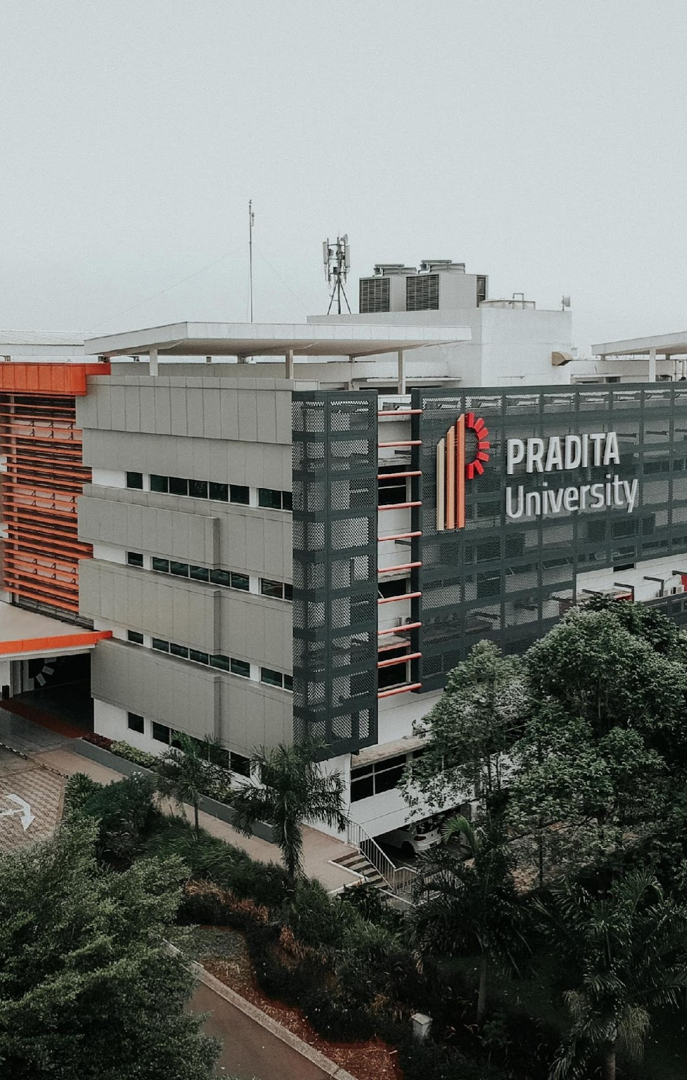
\includegraphics[width=\paperwidth]{../figures/building.png}
    };

    % Judul
    \node[anchor=center] at ([yshift=.1\textheight]current page.center) {
      \begin{minipage}{\textwidth}

        {\LARGE \textbf{Modul Kuliah -- IF231303}}\\[0.03\textheight]
        {\HUGE \textcolor{praditagreen}{
        \textbf{Arsitektur\vspace{10pt}\\
            Perangkat Lunak
        }}}\\[.05\textheight]
        {\LARGE \textbf{Alfa Yohannis}}\\[0.05\textheight]
      \end{minipage}
    };

    % Panel bawah
    \node[anchor=south west] at (
    current page.south west) {
      \begin{tikzpicture}[remember picture, overlay]
        \node[anchor=south west, fill=praditagreen, text=white, minimum width=\paperwidth, minimum height=.14\textheight, align=center, font=\Huge\bfseries] at (-.15,-.15) {
          Program Studi Teknologi Informasi\\
          Universitas Pradita
        };
      \end{tikzpicture}
    };
  \end{tikzpicture}
\end{titlepage}


  % Contents Page
  \tableofcontents

  % Sementara hanya Bab 2 yang dikompilasi agar render cepat.
  % Aktifkan kembali baris lain sebelum modul dicetak utuh.
  \chapter{Pengenalan Arsitektur Perangkat Lunak dan Client-Server}

\section*{Tujuan Pembelajaran}

\begin{enumerate}
  \item Menjelaskan arti arsitektur perangkat lunak beserta aspek yang
    membedakannya dari rancangan rinci.
  \item Membedakan tanggung jawab klien dari tanggung jawab server pada
    arsitektur client-server.
  \item Mengukur waktu bolak-balik satu permintaan dan perubahannya ketika
    jumlah klien bertambah.
\end{enumerate}

\section{Pendahuluan}

Setiap sistem perangkat lunak punya arsitektur, baik dirancang maupun tidak.
Arsitektur adalah susunan bagian-bagian besar sistem beserta aturan hubungan di
antaranya. Susunan itu menentukan hal-hal yang mahal diubah di kemudian hari,
misalnya batas antar modul dan cara modul berkomunikasi.

Yang membedakan arsitektur dari rancangan rinci adalah biaya perubahannya.
Mengganti nama sebuah fungsi murah. Memindahkan aturan bisnis dari satu bagian
ke bagian lain juga masih murah. Sebaliknya, memecah satu sistem menjadi
beberapa layanan terpisah menyentuh hampir seluruh berkas. Keputusan yang mahal
diubah itulah yang disebut keputusan arsitektural.

Bab ini membuka dengan pengertian arsitektur perangkat lunak beserta aspek yang
dinilainya, lalu menutup dengan bentuk pertama yang dibahas dalam modul ini,
yaitu client-server. Bentuk tersebut dipilih lebih dahulu karena hampir seluruh
bentuk lain pada bab-bab berikutnya tetap memakainya sebagai dasar. Pembahasan
mengikuti kerangka yang disusun oleh Richards dan
Ford~\cite{richards2020fundamentals}.

\section{Aspek yang Dinilai pada Sebuah Arsitektur}

Sebuah arsitektur tidak dinilai benar atau salah, melainkan sesuai atau tidak
sesuai dengan kebutuhan. Penilaiannya memakai sejumlah aspek, dan aspek-aspek
tersebut sering saling bertentangan. Tabel~\ref{tab:aspek} merangkum lima aspek
yang paling sering dipakai.

\begin{table}[htbp]
  \centering
  \caption{Lima aspek yang paling sering dipakai untuk menilai arsitektur}
  \label{tab:aspek}
  \begin{tabularx}{\textwidth}{|l|X|X|}
    \hline
    \textbf{Aspek} & \textbf{Pertanyaannya} & \textbf{Diukur dengan} \\
    \hline
    Kemudahan perawatan & Berapa banyak berkas berubah untuk satu permintaan perubahan? & Jumlah berkas dan baris \\
    \hline
    Kemampuan skala & Apa yang terjadi ketika jumlah pengguna naik sepuluh kali? & Latensi pada beban bertingkat \\
    \hline
    Kinerja & Berapa lama satu permintaan dilayani? & Median dan persentil ke-95 \\
    \hline
    Ketersediaan & Apa yang gagal ketika satu bagian mati? & Jumlah proses yang terhenti \\
    \hline
    Kemudahan pengujian & Berapa besar bagian yang dapat diuji tanpa infrastruktur? & Cakupan pengujian \\
    \hline
  \end{tabularx}
\end{table}

Aspek-aspek tersebut jarang dapat dipenuhi seluruhnya sekaligus. Menaikkan
kemampuan skala biasanya menurunkan kemudahan perawatan, sebab sistem harus
dipecah menjadi lebih banyak bagian. Menaikkan kinerja sering menurunkan
kemudahan pengujian, sebab jalan pintas mulai bermunculan. Pekerjaan seorang
arsitek karena itu bukan mencari susunan terbaik, melainkan memilih aspek mana
yang dikorbankan.

Setiap bab pada modul ini mengukur dua atau tiga aspek dari tabel tersebut, lalu
melaporkan angkanya. Cara itu dipakai agar perbandingan antar bentuk arsitektur
berdiri di atas angka, bukan di atas pendapat.

\section{Studi Kasus Singkat}

Tiga kejadian berikut menunjukkan bahwa keputusan arsitektural berakibat nyata,
bukan sekadar soal kerapian kode.

\textbf{Netflix.} Pada 2008 layanan Netflix berhenti cukup lama akibat kerusakan
pada basis data tunggalnya. Seluruh sistem saat itu berupa satu kesatuan, dan
kegagalan satu bagian menghentikan seluruhnya. Sesudah kejadian tersebut sistem
dipecah menjadi banyak layanan terpisah, sehingga kegagalan satu layanan tidak
lagi menghentikan yang lain.

\textbf{Healthcare.gov.} Pada peluncurannya tahun 2013 situs pendaftaran
asuransi kesehatan Amerika Serikat tersebut nyaris tidak dapat dipakai. Salah
satu sebabnya, sistem memanggil banyak sistem luar secara berurutan dan menunggu
seluruh jawabannya sebelum menampilkan halaman. Satu sistem luar yang lambat
membuat seluruh halaman ikut lambat.

\textbf{Sistem perbankan.} Sistem yang memproses transaksi secara berkelompok
pada akhir hari menunda pembaruan saldo sampai kelompok tersebut selesai
diproses. Perpindahan ke pemrosesan berbasis event membuat saldo diperbarui
segera setelah transaksi terjadi. Bab~9 membahas bentuk tersebut secara khusus.

Ketiganya memperlihatkan pola yang sama. Yang gagal bukan algoritmanya,
melainkan susunan bagian-bagiannya beserta cara mereka saling menunggu.

\section{Arsitektur Client-Server}

Client-server membagi sistem menjadi dua peran. Klien meminta, server melayani.
Gambar~\ref{fig:client-server} menunjukkan susunannya. Banyak klien memanggil
satu server, dan seluruh panah berawal dari klien.

\begin{figure}[htbp]
  \centering
  \begin{tikzpicture}[
    kotak/.style={draw, rounded corners=2pt, minimum width=1.8cm,
      minimum height=0.7cm, align=center, font=\scriptsize},
    server/.style={draw, rounded corners=3pt, minimum width=3.0cm,
      minimum height=1.4cm, align=center, font=\scriptsize, fill=praditagreen!15},
    panah/.style={-{Stealth[length=2mm]}, thick}
  ]
    \node[server] (srv) {\textbf{Server}\\
      {\tiny\mdseries menyimpan tabel kurs}\\
      {\tiny\mdseries menjalankan perhitungan}};

    \node[kotak, fill=blue!8, left=2.6cm of srv, yshift=1.15cm] (k1) {Klien 1};
    \node[kotak, fill=blue!8, left=2.6cm of srv] (k2) {Klien 2};
    \node[kotak, fill=blue!8, left=2.6cm of srv, yshift=-1.15cm] (k3) {Klien 3};

    \draw[panah] (k1.east) -- node[above, font=\tiny, pos=0.55] {permintaan} (srv.west);
    \draw[panah] (k2.east) -- (srv.west);
    \draw[panah] (k3.east) -- (srv.west);
  \end{tikzpicture}
  \caption{Banyak klien memanggil satu server. Seluruh permintaan berawal dari
    klien, dan server tidak pernah memanggil klien}
  \label{fig:client-server}
\end{figure}

Pembagian tersebut menentukan siapa menyimpan apa. Server menyimpan data
bersama dan menjalankan aturan bisnis. Klien menyimpan keadaan tampilan saja.
Karena tabel kurs hanya ada di server, memperbaruinya cukup dilakukan di satu
tempat, dan seluruh klien langsung memakai nilai baru tersebut.

Analogi yang mendekati adalah warung dengan satu kasir. Pembeli antre dan
memesan, kasir yang menghitung dan menyimpan uang. Pembeli tidak perlu tahu
harga pokok setiap barang, dan perubahan harga cukup diberitahukan kepada kasir.
Kelemahannya juga sama, yaitu ketika pembeli banyak, antrean memanjang walaupun
setiap pesanan sebenarnya cepat dilayani.

Listing~\ref{lst:penangan} memperlihatkan inti server pada contoh bab ini.
Server membaca parameter permintaan, menghitung, lalu membalas dalam bentuk
JavaScript Object Notation (JSON).

\begin{lstlisting}[style=PythonStyle, caption={Penanganan satu permintaan pada
  server, tersedia di \berkas{sources/chapter01/server.py}}, label=lst:penangan]
def do_GET(self):
  """Membaca parameter permintaan, menghitung, lalu membalas dalam JSON."""
  parameter = parse_qs(urlparse(self.path).query)
  asal = parameter.get("asal", ["USD"])[0]
  tujuan = parameter.get("tujuan", ["IDR"])[0]
  nominal = float(parameter.get("nominal", ["1"])[0])

  hasil = hitung_konversi(asal, tujuan, nominal)
  if hasil is None:
    self.kirim(404, {"galat": "Kurs tidak tersedia"})
  else:
    self.kirim(200, {"asal": asal, "tujuan": tujuan, "hasil": hasil})
\end{lstlisting}

Klien pada contoh tersebut sangat tipis. Klien hanya menyusun alamat, mengirim
permintaan, lalu menampilkan jawaban. Tidak ada tabel kurs dan tidak ada
perhitungan di sisi klien.

\section{Dua Biaya yang Melekat}

Pemisahan klien dan server menimbulkan dua biaya yang tidak dapat dihindari.
Keduanya menjadi bahan pengukuran pada latihan bab ini.

\textbf{Biaya perjalanan.} Setiap permintaan harus menempuh jaringan dua kali,
yaitu pergi dan pulang. Pada server di komputer yang sama biaya ini kecil, tetapi
tetap ada. Pada server yang berada di kota lain, biaya ini menjadi bagian
terbesar dari waktu tanggap, dan tidak dapat diperkecil dengan mempercepat
perhitungannya.

\textbf{Biaya antrean.} Satu server melayani banyak klien. Ketika permintaan
datang lebih cepat daripada kemampuan server melayaninya, sisanya menunggu.
Server pada contoh bab ini melayani satu permintaan pada satu waktu, sehingga
gejala tersebut muncul jelas begitu jumlah klien bertambah.

Tabel~\ref{tab:biaya-cs} merangkum hasil pengukuran nyata pada contoh bab ini.
Kolom terakhir memperlihatkan gejala antrean tersebut.

\begin{table}[htbp]
  \centering
  \caption{Latensi terhadap jumlah klien serentak pada server contoh}
  \label{tab:biaya-cs}
  \begin{tabularx}{\textwidth}{|X|l|l|}
    \hline
    \textbf{Jumlah klien serentak} & \textbf{Median (ms)} & \textbf{Terbesar (ms)} \\
    \hline
    1 & 0,240 & 8,027 \\
    \hline
    2 & 0,363 & 0,848 \\
    \hline
    4 & 0,777 & 1,748 \\
    \hline
    8 & 1,472 & 1011,138 \\
    \hline
    16 & 1,481 & 1019,625 \\
    \hline
  \end{tabularx}
\end{table}

Angka pada kolom terakhir melonjak tajam mulai delapan klien. Nilai median hanya
naik dari 0,24 menjadi 1,48 milidetik, sedangkan nilai terbesarnya mencapai
seribu milidetik. Sebagian permintaan karena itu menunggu sangat lama, sementara
sebagian besar lainnya tetap cepat. Gejala tersebut tidak terlihat bila yang
dilaporkan hanya nilai rata-rata, dan itulah alasan pengukuran pada modul ini
selalu menyertakan nilai terbesar atau persentil ke-95.

\section{Kelebihan dan Kekurangan}

Tabel~\ref{tab:untung-rugi-cs} merangkum untung rugi bentuk client-server.

\begin{table}[htbp]
  \centering
  \caption{Kelebihan dan kekurangan arsitektur client-server}
  \label{tab:untung-rugi-cs}
  \begin{tabularx}{\textwidth}{|X|X|}
    \hline
    \textbf{Kelebihan} & \textbf{Kekurangan} \\
    \hline
    Data bersama disimpan di satu tempat, sehingga pembaruan cukup sekali & Server menjadi satu-satunya titik yang bila mati menghentikan seluruh layanan \\
    \hline
    Aturan bisnis tidak dapat diubah dari sisi klien & Setiap permintaan menanggung biaya perjalanan jaringan \\
    \hline
    Klien menjadi ringan dan mudah diganti & Server menjadi antrean bersama ketika klien bertambah \\
    \hline
    Perangkat klien tidak perlu bertenaga besar & Menambah kemampuan server lebih mahal daripada menambah klien \\
    \hline
  \end{tabularx}
\end{table}

\section{Ringkasan}

Arsitektur adalah susunan bagian besar sistem beserta aturan hubungan di
antaranya. Yang membedakannya dari rancangan rinci adalah biaya perubahan.
Keputusan yang murah diubah bukan keputusan arsitektural, sedangkan keputusan
yang menyentuh hampir seluruh berkas termasuk di dalamnya.

Sebuah arsitektur dinilai memakai beberapa aspek yang saling bertentangan, yaitu
kemudahan perawatan, kemampuan skala, kinerja, ketersediaan, dan kemudahan
pengujian. Aspek-aspek tersebut jarang dapat dipenuhi seluruhnya sekaligus,
sehingga pekerjaan seorang arsitek adalah memilih aspek mana yang dikorbankan.

Ketiga studi kasus pada bab ini memperlihatkan pola yang sama. Yang gagal bukan
algoritmanya, melainkan susunan bagian-bagiannya beserta cara mereka saling
menunggu. Perbaikannya pun bukan mempercepat perhitungan, melainkan mengubah
susunannya.

Client-server membagi sistem menjadi peminta dan pelayan. Server menyimpan data
bersama dan menjalankan aturan bisnis, sedangkan klien menyimpan keadaan
tampilan saja. Pembagian tersebut membuat pembaruan data cukup dilakukan di satu
tempat, dan membuat aturan bisnis tidak dapat diubah dari sisi klien.

Pembagian itu menimbulkan dua biaya tetap, yaitu perjalanan jaringan dan antrean
di server. Pengukuran pada bab ini menunjukkan biaya antrean tidak terlihat pada
nilai median, tetapi tampak jelas pada nilai terbesar. Karena itu setiap
pengukuran pada modul ini melaporkan sebaran, bukan satu angka rata-rata.

\section{Latihan}

Ketiga latihan berikut memakai satu basis kode yang sama di
\berkas{sources/chapter01/}, tetapi menyasar tiga masalah yang berbeda.
Latihan~1 memeriksa pemisahan tanggung jawab. Latihan~2 mengukur biaya
perjalanan. Latihan~3 mengukur perilaku server ketika klien bertambah. Seluruh
pengukuran hanya dijalankan terhadap server milik sendiri, tidak terhadap
sistem milik pihak lain. Hasil setiap mahasiswa dapat berbeda, dan yang
dilaporkan adalah pola perbandingannya.

Server dijalankan lebih dahulu pada satu terminal seperti pada
Listing~\ref{lst:jalankan-server}, lalu skrip lainnya pada terminal kedua.

\begin{lstlisting}[language=bash, caption={Menjalankan server pada terminal pertama},
  label=lst:jalankan-server]
cd sources/chapter01
python server.py
\end{lstlisting}

\subsection*{Latihan 1: Memetakan Tanggung Jawab}

Latihan ini membuktikan bahwa klien tidak menyimpan maupun menghitung apa pun.
Langkah kerjanya sebagai berikut.

\begin{enumerate}
  \item Jalankan \texttt{python klien.py USD IDR 100} pada terminal kedua, lalu
    catat jawabannya.
  \item Buka \berkas{sources/chapter01/klien.py}, lalu cari tabel kurs di
    dalamnya.
  \item Ubah satu nilai pada tabel kurs di \berkas{sources/chapter01/server.py},
    jalankan ulang server, lalu jalankan klien tanpa mengubah apa pun.
  \item Matikan server, lalu jalankan klien sekali lagi dan catat yang terjadi.
\end{enumerate}

Tabel~\ref{tab:lat1cs-contoh} memperlihatkan bentuk pengisian yang diharapkan.

\begin{table}[htbp]
  \centering
  \caption{Contoh hasil Latihan 1 yang sudah terisi}
  \label{tab:lat1cs-contoh}
  \begin{tabularx}{\textwidth}{|X|l|X|}
    \hline
    \textbf{Pertanyaan} & \textbf{Jawaban} & \textbf{Bukti} \\
    \hline
    Klien menyimpan tabel kurs & tidak & Tidak ada kamus KURS di \texttt{klien.py} \\
    \hline
    Klien ikut berubah setelah kurs diubah & tidak & Jawaban berubah tanpa menyunting klien \\
    \hline
  \end{tabularx}
\end{table}

Isikan hasil pengamatan pada Tabel~\ref{tab:lat1cs-hasil}.

\begin{table}[htbp]
  \centering
  \caption{Lembar isian Latihan 1}
  \label{tab:lat1cs-hasil}
  \begin{tabularx}{\textwidth}{|X|l|X|}
    \hline
    \textbf{Pertanyaan} & \textbf{Jawaban} & \textbf{Bukti} \\
    \hline
    Klien menyimpan tabel kurs & \dots & \dots \\
    \hline
    Klien menghitung konversi & \dots & \dots \\
    \hline
    Klien ikut berubah setelah kurs diubah & \dots & \dots \\
    \hline
    Yang terjadi ketika server dimatikan & \multicolumn{2}{X|}{\dots} \\
    \hline
  \end{tabularx}
\end{table}

Jawab dua pertanyaan berikut. Pertama, jelaskan keuntungan menyimpan tabel kurs
hanya di server. Kedua, jelaskan kerugiannya berdasarkan yang terjadi ketika
server dimatikan.

\subsection*{Latihan 2: Mengukur Biaya Perjalanan}

Latihan ini mengukur waktu bolak-balik satu permintaan. Langkah kerjanya sebagai
berikut.

\begin{enumerate}
  \item Jalankan \texttt{python ukur\_latensi.py}, lalu catat kelima angka yang
    dilaporkan.
  \item Ulangi pengukuran sebanyak tiga kali.
  \item Bandingkan nilai terkecil dengan nilai terbesar pada setiap pengukuran.
  \item Tambahkan perhitungan berulang di dalam \texttt{hitung\_konversi} agar
    server bekerja lebih lama, lalu ukur kembali.
\end{enumerate}

Tabel~\ref{tab:lat2cs-contoh} memperlihatkan hasil satu kali pengukuran nyata.

\begin{table}[htbp]
  \centering
  \caption{Contoh hasil Latihan 2 yang sudah terisi}
  \label{tab:lat2cs-contoh}
  \begin{tabularx}{\textwidth}{|X|l|l|l|}
    \hline
    \textbf{Pengukuran} & \textbf{Median} & \textbf{Persentil ke-95} & \textbf{Terbesar} \\
    \hline
    Ke-1, 200 permintaan & 0,237 ms & 0,351 ms & 7,391 ms \\
    \hline
  \end{tabularx}
\end{table}

Isikan hasil pengukuran pada Tabel~\ref{tab:lat2cs-hasil}.

\begin{table}[htbp]
  \centering
  \caption{Lembar isian Latihan 2}
  \label{tab:lat2cs-hasil}
  \begin{tabularx}{\textwidth}{|X|l|l|l|}
    \hline
    \textbf{Pengukuran} & \textbf{Median} & \textbf{Persentil ke-95} & \textbf{Terbesar} \\
    \hline
    Ke-1 & \dots & \dots & \dots \\
    \hline
    Ke-2 & \dots & \dots & \dots \\
    \hline
    Ke-3 & \dots & \dots & \dots \\
    \hline
    Setelah server dibuat lebih lambat & \dots & \dots & \dots \\
    \hline
  \end{tabularx}
\end{table}

Jawab dua pertanyaan berikut dengan menunjuk angka pada tabel. Pertama, nilai
terbesar pada pengukuran pertama jauh melebihi mediannya, sehingga jelaskan
sebabnya. Kedua, jelaskan bagian mana dari waktu tersebut yang tetap ada
walaupun perhitungan di server dipercepat.

\subsection*{Latihan 3: Menambah Jumlah Klien}

Latihan ini membuktikan bahwa server adalah antrean bersama. Langkah kerjanya
sebagai berikut.

\begin{enumerate}
  \item Jalankan \texttt{python ukur\_beban.py}, lalu catat median dan nilai
    terbesar pada setiap jumlah klien.
  \item Tandai jumlah klien saat nilai terbesar mulai melonjak.
  \item Bandingkan pertumbuhan median terhadap pertumbuhan nilai terbesar.
  \item Jelaskan mengapa keduanya tumbuh dengan pola yang berbeda.
\end{enumerate}

Tabel~\ref{tab:lat3cs-contoh} memperlihatkan hasil satu kali pengukuran nyata.

\begin{table}[htbp]
  \centering
  \caption{Contoh hasil Latihan 3 yang sudah terisi}
  \label{tab:lat3cs-contoh}
  \begin{tabularx}{\textwidth}{|X|l|l|}
    \hline
    \textbf{Jumlah klien} & \textbf{Median (ms)} & \textbf{Terbesar (ms)} \\
    \hline
    4 & 0,777 & 1,748 \\
    \hline
    8 & 1,472 & 1011,138 \\
    \hline
  \end{tabularx}
\end{table}

Isikan hasil pengukuran pada Tabel~\ref{tab:lat3cs-hasil}.

\begin{table}[htbp]
  \centering
  \caption{Lembar isian Latihan 3}
  \label{tab:lat3cs-hasil}
  \begin{tabularx}{\textwidth}{|X|l|l|}
    \hline
    \textbf{Jumlah klien} & \textbf{Median (ms)} & \textbf{Terbesar (ms)} \\
    \hline
    1 & \dots & \dots \\
    \hline
    2 & \dots & \dots \\
    \hline
    4 & \dots & \dots \\
    \hline
    8 & \dots & \dots \\
    \hline
    16 & \dots & \dots \\
    \hline
    Jumlah klien saat lonjakan mulai & \multicolumn{2}{l|}{\dots} \\
    \hline
  \end{tabularx}
\end{table}

Jawab tiga pertanyaan berikut dengan menunjuk angka pada tabel. Pertama, median
tumbuh perlahan sedangkan nilai terbesar melonjak, sehingga jelaskan apa yang
dialami sebagian kecil permintaan tersebut. Kedua, jelaskan mengapa gejala itu
hilang bila hanya nilai rata-rata yang dilaporkan. Ketiga, dengan menggabungkan
hasil ketiga latihan, sebutkan aspek dari Tabel~\ref{tab:aspek} yang paling
tertekan pada arsitektur client-server beserta angka yang menjadi dasarnya.

  \chapter{Layered Architecture}
\label{bab:lapisan}

\section*{Tujuan Pembelajaran}

\begin{enumerate}
  \item Menjelaskan pembagian tanggung jawab pada keempat lapisan \textit{layered
    architecture} dan arah ketergantungan yang berlaku di antaranya.
  \item Membedakan lapisan tertutup dari lapisan terbuka, lalu menentukan kapan
    masing-masing bentuk layak dipilih.
  \item Mengukur jumlah fungsi penerus, pelanggaran arah ketergantungan, dan
    selisih waktu antara kedua bentuk pada satu aplikasi yang sama.
\end{enumerate}

\section{Pendahuluan}

\textit{Layered architecture} menata sebuah aplikasi menjadi beberapa lapisan
yang bertumpuk. Setiap lapisan mengerjakan satu jenis urusan teknis, lalu
memanggil lapisan di bawahnya bila membutuhkan sesuatu. Bentuk ini juga dikenal
sebagai arsitektur \textit{n-tier}~\cite{microsoft2024ntier}. Bentuk ini menjadi pilihan pertama bagi
sebagian besar sistem, dan sering dipakai tanpa pertimbangan panjang ketika tim
belum memutuskan arsitektur lain.

Fowler~\cite{fowler2015layering} mencatat bahwa pembagian menjadi tampilan,
domain, dan data merupakan pembagian yang paling sering dipakai, sekaligus yang
paling sering dipakai tanpa alasan yang dipikirkan.

Salah satu alasan pemakaiannya bersifat organisasi, bukan teknis. Pembagian
lapisan mengikuti pembagian kerja yang sudah ada di banyak tim pengembang. Ada
yang mengerjakan antarmuka, ada yang mengerjakan aturan bisnis, dan ada yang
mengerjakan basis data. Struktur tim tersebut memetakan diri dengan rapi ke
struktur lapisan, sehingga setiap orang tahu berkas mana yang menjadi
tanggung jawabnya.

Kemudahan itu ada harganya. Ketika aplikasi membesar, pemisahan yang tadinya
menolong justru memperlambat perubahan. Satu fitur baru sering menyentuh
keempat lapisan sekaligus. Bab ini membahas pembagian lapisan, aturan
ketergantungan di antaranya, serta pilihan antara lapisan tertutup dan lapisan
terbuka. Pembahasan mengikuti kerangka yang disusun oleh Richards dan
Ford~\cite{richards2020fundamentals}.

\section{Pembagian Lapisan}

Bentuk baku \textit{layered architecture} terdiri atas empat lapisan.
Gambar~\ref{fig:lapisan-empat} menunjukkan susunannya beserta arah panggilan
yang diizinkan. Panah hanya menunjuk ke bawah, dan tidak ada panah yang
melompati satu lapisan.

\begin{figure}[htbp]
  \centering
  \begin{tikzpicture}[
    lapis/.style={draw, rounded corners=2pt, minimum width=0.62\textwidth,
      minimum height=1.05cm, align=center, font=\scriptsize},
    panah/.style={-{Stealth[length=2mm]}, thick}
  ]
    \node[lapis, fill=blue!8] (pres) {\textbf{Lapisan Presentasi}\\
      {\tiny\mdseries Menerima masukan, menampilkan hasil}};
    \node[lapis, fill=blue!8, below=0.55cm of pres] (bis) {\textbf{Lapisan Bisnis}\\
      {\tiny\mdseries Memeriksa dan menjalankan aturan bisnis}};
    \node[lapis, fill=blue!8, below=0.55cm of bis] (per) {\textbf{Lapisan Persistensi}\\
      {\tiny\mdseries Menerjemahkan data simpanan menjadi objek}};
    \node[lapis, fill=green!10, below=0.55cm of per] (bas) {\textbf{Lapisan Basis Data}\\
      {\tiny\mdseries Menyimpan data secara permanen}};

    \draw[panah] (pres) -- (bis);
    \draw[panah] (bis) -- (per);
    \draw[panah] (per) -- (bas);
  \end{tikzpicture}
  \caption{Empat lapisan baku beserta arah panggilan yang diizinkan}
  \label{fig:lapisan-empat}
\end{figure}

\textbf{Lapisan presentasi} menangani segala hal yang dilihat pengguna. Lapisan
ini menerima masukan, memanggil lapisan bisnis, lalu menampilkan hasilnya.
Lapisan ini tidak mengetahui asal data maupun cara data disimpan. Contohnya
menyusun teks \texttt{100 USD = 1.625.000 IDR} lengkap dengan pemisah ribuan,
menampilkan pesan galat ketika nominal ditolak, dan mengubah daftar kurs menjadi
baris-baris teks. Bila layar diganti menjadi API, seluruh isi lapisan ini
dibuang dan ditulis ulang.

\textbf{Lapisan bisnis} memuat aturan yang membuat sistem tersebut bernilai.
Pemeriksaan kelayakan, perhitungan, dan keputusan proses berada di sini.
Lapisan ini tidak mengetahui bentuk antarmuka maupun bentuk tabel basis data.
Contohnya menolak nominal yang bernilai nol atau negatif, menolak nominal yang
melewati batas wajar, memeriksa token pemanggil, dan memeriksa apakah peran
pemanggil berhak membaca kurs jual. Seluruh aturan tersebut tetap berlaku
walaupun layarnya diganti.

\textbf{Lapisan persistensi} menjembatani objek di dalam program dengan baris di
dalam basis data. Kueri Structured Query Language (SQL) ditulis di lapisan ini,
sehingga lapisan bisnis tidak perlu mengetahui nama tabel. Contohnya menjalankan
kueri pencarian satu kurs, mengubah baris hasil kueri menjadi tupel siap pakai,
dan mengembalikan nilai kosong ketika pasangan mata uang tidak ditemukan. Bila
basis datanya berganti, hanya isi lapisan inilah yang ditulis ulang.

\textbf{Lapisan basis data} menyimpan data secara permanen. Lapisan ini biasanya
berupa perangkat lunak tersendiri, bukan kode yang ditulis tim pengembang.
Contohnya tabel \texttt{kurs} beserta kolom \texttt{nilai} dan
\texttt{margin}, kunci utama berupa pasangan kode mata uang, serta aturan bahwa
satu pasangan hanya boleh muncul satu kali. Keputusan menyimpan margin pada
kolom terpisah diambil di lapisan ini, dan keputusan itulah yang memungkinkan
kurs referensi dibaca tanpa ikut membuka marginnya.

Pembagian tersebut memberi satu keuntungan yang jelas. Perubahan pada satu
urusan teknis tertahan di satu lapisan. Penggantian basis data, misalnya, cukup
menyentuh lapisan persistensi selama bentuk objek yang dikembalikannya tetap.
Tabel~\ref{tab:tanggung-jawab} merangkum tanggung jawab dan larangan setiap
lapisan.

\begin{table}[htbp]
  \centering
  \caption{Tanggung jawab dan larangan setiap lapisan}
  \label{tab:tanggung-jawab}
  \begin{tabularx}{\textwidth}{|l|X|X|}
    \hline
    \textbf{Lapisan} & \textbf{Tanggung jawab} & \textbf{Tidak boleh mengetahui} \\
    \hline
    Presentasi & Menerima masukan dan menampilkan hasil & Nama tabel, kueri, sumber data \\
    \hline
    Bisnis & Memeriksa aturan dan menghitung hasil & Bentuk antarmuka, bentuk tabel \\
    \hline
    Persistensi & Menerjemahkan baris menjadi objek & Aturan bisnis, kebutuhan tampilan \\
    \hline
    Basis Data & Menyimpan data secara permanen & Seluruh lapisan di atasnya \\
    \hline
  \end{tabularx}
\end{table}

Agar pembagian tersebut tidak berhenti sebagai daftar, Tabel~\ref{tab:contoh-lapisan}
menunjukkan isi setiap lapisan pada aplikasi kurs yang dipakai sepanjang bab
ini. Perhatikan bahwa satu kalimat kebutuhan biasanya jatuh ke satu lapisan
saja.

\begin{table}[htbp]
  \centering
  \caption{Contoh isi setiap lapisan pada aplikasi kurs}
  \label{tab:contoh-lapisan}
  \begin{tabularx}{\textwidth}{|l|X|X|}
    \hline
    \textbf{Lapisan} & \textbf{Contoh isinya} & \textbf{Kalimat kebutuhan} \\
    \hline
    Presentasi & Menyusun teks \texttt{100 USD = 1.625.000 IDR} & Hasil ditampilkan dengan pemisah ribuan \\
    \hline
    Bisnis & Menolak nominal nol, memeriksa token dan peran & Hanya staf boleh melihat kurs jual \\
    \hline
    Persistensi & Mengubah baris tabel menjadi tupel & Kurs disimpan per pasangan mata uang \\
    \hline
    Basis Data & Tabel \texttt{kurs} beserta kolom \texttt{margin} & Margin disimpan terpisah dari nilai referensi \\
    \hline
  \end{tabularx}
\end{table}

Uji cepat untuk menempatkan sebuah kebutuhan cukup satu pertanyaan. Bila
kebutuhan tersebut tetap berlaku walaupun aplikasi berganti dari layar menjadi
API, kebutuhan itu milik lapisan bisnis. Bila kebutuhan tersebut hilang ketika
layarnya diganti, kebutuhan itu milik lapisan presentasi.

\section{Aturan Ketergantungan}

Aturan pokok \textit{layered architecture} hanya satu. Sebuah lapisan boleh
memanggil lapisan tepat di bawahnya, dan tidak boleh memanggil ke atas. Aturan
itu terdengar sederhana, tetapi menentukan hampir seluruh sifat arsitektur ini.

Analogi yang mendekati adalah loket pembayaran uang kuliah di kampus.
Mahasiswa berbicara kepada petugas loket, petugas loket berbicara kepada bagian
keuangan, lalu bagian keuangan berbicara kepada bank. Mahasiswa tidak menelepon
bank secara langsung, dan bank tidak memanggil mahasiswa. Setiap pihak hanya
mengenal tetangga terdekatnya.

Aturan tersebut punya dua konsekuensi praktis. Pertama, satu lapisan dapat
diganti tanpa menyentuh lapisan lain, selama bentuk panggilannya tetap sama.
Jadi, tidak perlu mengubah lapisan lain. Kedua, satu permintaan yang sederhana
tetap harus melewati seluruh lapisan, walaupun sebagian lapisan tidak
mengerjakan apa pun.

Konsekuensi kedua itulah yang menimbulkan persoalan berikutnya. Pertanyaannya,
apakah setiap permintaan benar-benar wajib melewati semua lapisan.

\section{Lapisan Tertutup dan Lapisan Terbuka}

Dua jawaban atas pertanyaan tersebut menghasilkan dua bentuk yang berbeda.
Gambar~\ref{fig:tertutup-terbuka} menunjukkan keduanya berdampingan.

\begin{figure}[htbp]
  \centering
  \begin{tikzpicture}[
    lapis/.style={draw, rounded corners=2pt, minimum width=3.1cm,
      minimum height=0.85cm, align=center, font=\scriptsize},
    panah/.style={-{Stealth[length=2mm]}, thick},
    lompat/.style={-{Stealth[length=2mm]}, thick, red!70, dashed}
  ]
    % Kiri: tertutup
    \node[lapis, fill=blue!8] (p1) {Presentasi};
    \node[lapis, fill=blue!8, below=0.5cm of p1] (b1) {Bisnis};
    \node[lapis, fill=blue!8, below=0.5cm of b1] (s1) {Persistensi};
    \node[font=\scriptsize\bfseries, above=0.25cm of p1] {Lapisan tertutup};
    \draw[panah] (p1) -- (b1);
    \draw[panah] (b1) -- (s1);

    % Kanan: terbuka
    \node[lapis, fill=blue!8, right=2.6cm of p1] (p2) {Presentasi};
    \node[lapis, fill=praditagreen!15, below=0.5cm of p2] (b2) {Bisnis};
    \node[lapis, fill=blue!8, below=0.5cm of b2] (s2) {Persistensi};
    \node[font=\scriptsize\bfseries, above=0.25cm of p2] {Lapisan terbuka};
    \draw[panah] (p2) -- (b2);
    \draw[panah] (b2) -- (s2);
    \draw[lompat] (p2.east) to[out=-25, in=25] node[right, font=\tiny, align=left]
      {jalur\\pintas} (s2.east);
  \end{tikzpicture}
  \caption{Lapisan tertutup mewajibkan setiap panggilan melewati lapisan bisnis,
    sedangkan lapisan terbuka mengizinkan jalur pintas}
  \label{fig:tertutup-terbuka}
\end{figure}

Pada \textbf{lapisan tertutup}, setiap panggilan wajib melewati seluruh lapisan
tanpa perkecualian. Susunan ini menjaga arah ketergantungan tetap bersih.
Harganya muncul pada permintaan yang tidak punya aturan bisnis sama sekali.
Lapisan bisnis lalu hanya meneruskan panggilan tanpa menambahkan apa pun.

Keadaan tersebut dikenal sebagai \textit{architecture sinkhole anti-pattern},
yaitu permintaan yang mengalir melewati beberapa lapisan tanpa satu pun lapisan
mengerjakan sesuatu. Permintaan hanya turun untuk mengambil data, lalu naik
kembali tanpa diolah~\cite{richards2020fundamentals}. Keadaan ini hampir tidak
mungkin dihapus sepenuhnya, sehingga yang diusahakan adalah menekan jumlahnya,
bukan menghilangkannya. Yang perlu diperiksa adalah apakah lapisan bisnis lebih
sering meneruskan panggilan daripada mengerjakan sesuatu.
Analogi yang mendekati adalah surat pengantar yang harus melewati tiga meja.
Meja pertama membaca isinya dan memutuskan, sedangkan meja kedua dan ketiga
hanya membubuhkan cap lalu meneruskan. Ketiga meja tersebut sama-sama menambah
waktu, tetapi hanya satu yang menambah nilai. Bila keadaan itu dibiarkan,
prosedurnya terlihat rapi di atas kertas namun tidak berguna dalam praktik.


Pada \textbf{lapisan terbuka}, permintaan tanpa aturan bisnis boleh memangkas
satu lompatan. Lapisan presentasi memanggil lapisan persistensi secara langsung.
Bentuk ini memangkas kode penerus, tetapi menimbulkan ketergantungan baru.

\section{Kapan Jalan Pintas Dapat Dibenarkan}

Pertanyaan yang sebenarnya bukan apakah jalan pintas lebih cepat, melainkan
apakah ada tuntutan bisnis yang ikut dilewati. Contoh pada bab ini memakai dua
permintaan yang membaca tabel yang sama, tetapi tuntutan bisnisnya berbeda.

\textbf{Kurs referensi} adalah nilai tukar yang diterbitkan untuk umum. Bank
Indonesia menerbitkan angka semacam itu setiap hari kerja dengan nama Jakarta
Interbank Spot Dollar Rate (JISDOR), dan siapa pun boleh
membacanya~\cite{bi2026kurs}. Tidak ada
tuntutan bisnis yang berlaku pada pembacaan tersebut.

\textbf{Kurs jual} adalah kurs referensi ditambah margin milik bank. Margin
adalah informasi komersial, dan tuntutan bisnisnya menyatakan hanya staf yang
boleh membacanya. Pemeriksaan siapa pemanggilnya dan apakah pemanggil tersebut
berhak karena itu wajib dijalankan.

Kedua permintaan tersebut membaca tabel yang sama, sehingga tabel bukan yang
menentukan. Yang menentukan adalah tuntutan bisnis yang melekat pada masing-masing
permintaan. Tabel~\ref{tab:dua-permintaan} merangkum perbedaannya.

\begin{table}[htbp]
  \centering
  \caption{Dua permintaan pada tabel yang sama dengan tuntutan bisnis berbeda}
  \label{tab:dua-permintaan}
  \begin{tabularx}{\textwidth}{|l|X|X|}
    \hline
    \textbf{Permintaan} & \textbf{Tuntutan bisnis} & \textbf{Jalan pintas} \\
    \hline
    Kurs referensi & Tidak ada, data memang untuk umum & Dapat dibenarkan \\
    \hline
    Kurs jual & Autentikasi dan otorisasi, sebab memuat margin & Tidak dapat dibenarkan \\
    \hline
  \end{tabularx}
\end{table}

Listing~\ref{lst:penerus} memperlihatkan fungsi penerus pada kurs referensi.
Fungsi tersebut memang tidak menambahkan apa pun, dan itu wajar.

\begin{lstlisting}[style=PythonStyle, caption={Fungsi penerus yang wajar,
  tersedia di \berkas{sources/chapter02/aplikasi_tertutup.py}},
  label=lst:penerus]
def susun_kurs_referensi():
  """Meneruskan panggilan tanpa menambahkan apa pun.

  Kurs referensi memang diterbitkan untuk umum, meniru JISDOR yang diumumkan
  Bank Indonesia setiap hari kerja. Tidak ada tuntutan bisnis yang berlaku,
  sehingga fungsi ini murni penerus.
  """
  return daftar_kurs_referensi()
\end{lstlisting}

Bandingkan dengan Listing~\ref{lst:bisnis}. Fungsi kedua ini menjalankan dua
pemeriksaan sebelum data diberikan, dan kedua pemeriksaan itulah yang hilang
bila lapisan bisnis dilewati.

\begin{lstlisting}[style=PythonStyle, caption={Pemeriksaan yang dituntut lapisan
  bisnis, tersedia di \berkas{sources/chapter02/aplikasi_tertutup.py}},
  label=lst:bisnis]
def susun_kurs_jual(token):
  """Memeriksa autentikasi dan otorisasi sebelum kurs jual diberikan.

  Kurs jual memuat margin, dan margin adalah informasi komersial. Tuntutan
  bisnisnya menyatakan hanya staf yang boleh membacanya. Tuntutan itulah yang
  ikut hilang bila lapisan bisnis dilewati.
  """
  pengguna = autentikasi.periksa_token(token)
  if pengguna is None:
    raise PermissionError("Token tidak dikenali")
  if not autentikasi.boleh_membaca(pengguna):
    raise PermissionError(f"Peran {pengguna['peran']} tidak berhak membaca kurs jual")
  return daftar_kurs_jual()
\end{lstlisting}

Pada versi terbuka, lapisan presentasi memanggil \texttt{daftar\_jual} secara
langsung. Pemanggil tidak perlu menyerahkan token, dan margin ikut terbaca
siapa pun. Jalan pintas tersebut memang lebih cepat, sebab dua pemeriksaan
tidak dijalankan. Kecepatan itu dibeli dengan melepas tuntutan bisnis.
Kasus berikut memperlihatkan akibatnya. Sebuah tim menambahkan halaman
perbandingan kurs agar pengunjung dapat melihat nilai tukar tanpa masuk. Halaman
tersebut dibangun cepat dengan memanggil lapisan persistensi secara langsung,
dan pada tahap itu keputusannya benar, sebab yang ditampilkan hanya kurs
referensi. Beberapa bulan kemudian muncul permintaan menampilkan kurs jual pada
halaman yang sama. Fungsi yang dipakai tinggal diganti, sebab jalurnya sudah
terbuka. Sejak saat itu margin bank terbaca siapa pun tanpa satu pun pemeriksaan
dijalankan, dan tidak ada yang menyadarinya karena tidak ada galat yang muncul.

Pola kegagalan tersebut khas. Jalan pintas dibuat untuk data yang memang publik,
lalu belakangan dipakai ulang untuk data yang tidak publik. Karena itu jalan
pintas sebaiknya dicatat beserta alasannya, agar pemakaian berikutnya diperiksa
ulang, bukan diteruskan begitu saja.


Satu hal lain sering terlupakan. Lapisan mana yang tertutup dan lapisan mana
yang terbuka wajib dicatat dan disepakati satu tim. Tanpa catatan tersebut,
setiap orang menebak sendiri aturan yang berlaku, dan sistem berakhir dengan
ketergantungan yang rapat serta sulit diuji.

\section{Kelebihan dan Kekurangan}

Tabel~\ref{tab:untung-rugi} merangkum untung rugi kedua bentuk tersebut.
Perbandingan ini menjadi bahan pertimbangan sebelum memilih salah satunya.

\begin{table}[htbp]
  \centering
  \caption{Perbandingan lapisan tertutup dan lapisan terbuka}
  \label{tab:untung-rugi}
  \begin{tabularx}{\textwidth}{|l|X|X|}
    \hline
    \textbf{Aspek} & \textbf{Lapisan tertutup} & \textbf{Lapisan terbuka} \\
    \hline
    Arah ketergantungan & Bersih, hanya ke lapisan tepat di bawah & Presentasi ikut mengenal persistensi \\
    \hline
    Jumlah kode & Bertambah oleh fungsi penerus & Lebih sedikit \\
    \hline
    Kecepatan & Satu lompatan lebih banyak per permintaan & Satu lompatan lebih sedikit \\
    \hline
    Dampak perubahan & Tertahan di satu lapisan & Dapat merambat ke lapisan presentasi \\
    \hline
    Cocok untuk & Sistem dengan aturan bisnis padat & Pembacaan sederhana tanpa aturan bisnis \\
    \hline
  \end{tabularx}
\end{table}

Kelebihan utama \textit{layered architecture} secara umum ada tiga. Pembagian
kerja menjadi jelas, pengujian setiap lapisan dapat berdiri sendiri, dan
penggantian satu teknologi tidak menyentuh seluruh sistem. Ketiganya membuat
bentuk ini cocok untuk sistem berukuran kecil sampai menengah.

Kekurangannya muncul pada sistem besar. Satu fitur baru sering menyentuh
keempat lapisan sekaligus, sehingga tidak ada satu bagian pun yang dapat
di-\textit{deploy} sendiri. Selain itu seluruh lapisan tumbuh bersama-sama,
sehingga sistem tetap berupa satu kesatuan yang harus dirilis sekaligus.

\section{Ringkasan}

\textit{Layered architecture} membagi aplikasi menjadi empat lapisan, yaitu
presentasi, bisnis, persistensi, dan basis data. Setiap lapisan mengerjakan satu
jenis urusan teknis, lalu memanggil lapisan di bawahnya. Pembagian tersebut
mengikuti pembagian kerja yang sudah ada di banyak tim pengembang, dan itulah
salah satu alasan bentuk ini banyak dipakai.

Aturan pokoknya hanya satu, yaitu panggilan hanya boleh mengarah ke bawah.
Aturan itu menjaga agar perubahan pada satu urusan teknis tertahan di satu
lapisan. Penggantian basis data cukup menyentuh lapisan persistensi, selama
bentuk objek yang dikembalikannya tidak berubah.

Aturan yang sama menimbulkan biaya pada permintaan sederhana. Permintaan yang
tidak punya aturan bisnis tetap harus melewati lapisan bisnis, sehingga muncul
fungsi yang hanya meneruskan panggilan. Bila fungsi penerus sudah lebih banyak
daripada fungsi yang benar-benar bekerja, susunan lapisannya perlu ditinjau.

Lapisan terbuka mengizinkan jalur pintas untuk permintaan tanpa aturan bisnis.
Pengukuran seratus putaran pada latihan bab ini menunjukkan jalur pintas memang
lebih cepat, yaitu menang pada sembilan puluh satu putaran. Kecepatan itu
berasal dari dua pemeriksaan yang tidak dijalankan, bukan dari algoritma yang
lebih baik.

Pilihan antara keduanya karena itu bukan soal kecepatan, melainkan soal ada
tidaknya tuntutan bisnis yang ikut dilewati. Kurs referensi memang diterbitkan
untuk umum, sehingga jalan pintas padanya dapat dibenarkan. Kurs jual memuat
margin, dan tuntutan bisnisnya menyatakan hanya staf yang boleh membacanya,
sehingga jalan pintas padanya tidak dapat dibenarkan walaupun terbukti lebih
cepat. Keputusan diambil dengan membaca tuntutan bisnis setiap permintaan,
bukan dengan mengikuti kebiasaan.


\section{Latihan}

Ketiga latihan berikut memakai satu basis kode yang sama di
\berkas{sources/chapter02/}, tetapi menyasar tiga masalah yang berbeda.
Latihan~1 memeriksa lapisan yang tidak bekerja. Latihan~2 memeriksa arah
ketergantungan yang dilanggar. Latihan~3 mengukur biaya waktu satu lompatan
antar lapisan. Penilaian didasarkan pada kelengkapan tabel hasil dan ketepatan
jawaban analisisnya, bukan pada kecepatan pengerjaan. Hasil pengukuran setiap
mahasiswa akan berbeda, dan yang dilaporkan adalah pola perbandingannya, bukan
angka persisnya.

Seluruh latihan dijalankan seperti pada Listing~\ref{lst:persiapan}.

\begin{lstlisting}[language=bash, caption={Persiapan sebelum ketiga latihan},
  label=lst:persiapan]
cd sources/chapter02
python basis_data.py
\end{lstlisting}

\subsection*{Latihan 1: Menghitung Fungsi Penerus}

Latihan ini membuktikan berapa besar bagian lapisan bisnis yang hanya
meneruskan panggilan. Perbandingan tersebut sebenarnya dihitung dari jumlah
permintaan. Pada aplikasi sekecil ini setiap fungsi melayani tepat satu jalur
permintaan, sehingga menghitung fungsi sudah cukup mewakili. Langkah kerjanya
sebagai berikut.

\begin{enumerate}
  \item Jalankan \texttt{python periksa\_lapisan.py aplikasi\_tertutup.py}, lalu
    catat baris \texttt{Fungsi penerus} dan \texttt{Bagian penerus}.
  \item Jalankan perintah yang sama untuk \texttt{aplikasi\_terbuka.py}, lalu
    catat kedua baris tersebut.
  \item Buka kedua berkas, lalu periksa tubuh setiap fungsi yang dilaporkan
    sebagai penerus.
  \item Bandingkan bagian penerus pada kedua berkas, lalu nilai apakah lapisan
    bisnis lebih banyak bekerja daripada meneruskan.
\end{enumerate}

Tabel~\ref{tab:lat1-contoh} memperlihatkan hasil satu kali pemeriksaan nyata.

\begin{table}[htbp]
  \centering
  \caption{Contoh hasil Latihan 1 yang sudah terisi}
  \label{tab:lat1-contoh}
  \begin{tabularx}{\textwidth}{|X|l|l|l|}
    \hline
    \textbf{Berkas} & \textbf{Fungsi} & \textbf{Penerus} & \textbf{Bagian} \\
    \hline
    \texttt{aplikasi\_tertutup.py} & 12 & 1 & 8,3 persen \\
    \hline
    \texttt{aplikasi\_terbuka.py} & 6 & 0 & 0,0 persen \\
    \hline
  \end{tabularx}
\end{table}

Isikan hasil pemeriksaan pada Tabel~\ref{tab:lat1-hasil}.

\begin{table}[htbp]
  \centering
  \caption{Lembar isian Latihan 1}
  \label{tab:lat1-hasil}
  \begin{tabularx}{\textwidth}{|X|l|l|l|}
    \hline
    \textbf{Berkas} & \textbf{Fungsi} & \textbf{Penerus} & \textbf{Bagian} \\
    \hline
    \texttt{aplikasi\_tertutup.py} & \dots & \dots & \dots \\
    \hline
    \texttt{aplikasi\_terbuka.py} & \dots & \dots & \dots \\
    \hline
    Nama fungsi penerus & \multicolumn{3}{l|}{\dots} \\
    \hline
  \end{tabularx}
\end{table}

Jawab dua pertanyaan berikut dengan menunjuk angka pada tabel. Pertama, pada
versi tertutup, apakah lapisan bisnis lebih banyak bekerja daripada sekadar
meneruskan panggilan. Kedua, satu-satunya fungsi penerus yang tersisa melayani
kurs referensi, sehingga jelaskan mengapa keberadaan fungsi tersebut tetap
dapat dibenarkan.

\subsection*{Latihan 2: Menemukan Pelanggaran Arah Ketergantungan}

Latihan ini membuktikan bahwa jalur pintas menimbulkan ketergantungan baru.
Skrip \texttt{periksa\_lapisan.py} menghitung selisih indeks lapisan antara
pemanggil dan yang dipanggil, lalu menandai selisih dua atau lebih sebagai
pelanggaran. Langkah kerjanya sebagai berikut.

\begin{enumerate}
  \item Jalankan \texttt{python periksa\_lapisan.py} untuk kedua berkas
    aplikasi, lalu catat baris \texttt{Pelanggaran arah}.
  \item Salin nama fungsi pemanggil dan fungsi yang dipanggil pada setiap
    pelanggaran, beserta nama lapisannya.
  \item Buka \berkas{sources/chapter02/aplikasi_terbuka.py}, lalu temukan baris
    yang menimbulkan kedua pelanggaran tersebut.
  \item Jalankan \texttt{python aplikasi\_terbuka.py}, lalu perhatikan bahwa
    kurs jual terbaca tanpa token apa pun.
  \item Jalankan \texttt{python aplikasi\_tertutup.py USD IDR 100}, lalu
    bandingkan perlakuannya terhadap token yang tidak dikenali.
\end{enumerate}

Tabel~\ref{tab:lat2-contoh} memperlihatkan hasil satu kali pemeriksaan nyata.

\begin{table}[htbp]
  \centering
  \caption{Contoh hasil Latihan 2 yang sudah terisi}
  \label{tab:lat2-contoh}
  \begin{tabularx}{\textwidth}{|l|l|X|}
    \hline
    \textbf{Berkas} & \textbf{Pelanggaran} & \textbf{Rincian} \\
    \hline
    \texttt{aplikasi\_tertutup.py} & 0 & tidak ada \\
    \hline
    \texttt{aplikasi\_terbuka.py} & 2 & \texttt{tampilkan\_referensi} dan \texttt{tampilkan\_jual} memanggil lapisan persistensi langsung \\
    \hline
  \end{tabularx}
\end{table}

Isikan hasil pemeriksaan pada Tabel~\ref{tab:lat2-hasil}.

\begin{table}[htbp]
  \centering
  \caption{Lembar isian Latihan 2}
  \label{tab:lat2-hasil}
  \begin{tabularx}{\textwidth}{|l|l|X|}
    \hline
    \textbf{Berkas} & \textbf{Pelanggaran} & \textbf{Rincian} \\
    \hline
    \texttt{aplikasi\_tertutup.py} & \dots & \dots \\
    \hline
    \texttt{aplikasi\_terbuka.py} & \dots & \dots \\
    \hline
    Setelah fungsi baru ditambahkan & \dots & \dots \\
    \hline
  \end{tabularx}
\end{table}

Jawab tiga pertanyaan berikut dengan menunjuk isi tabel. Pertama, kedua
pelanggaran tersebut tidak sama beratnya, sehingga jelaskan mana yang dapat
dibenarkan dan mana yang tidak, beserta alasannya. Kedua, jelaskan apa yang
hilang ketika \texttt{tampilkan\_jual} memanggil lapisan persistensi langsung.
Ketiga, jelaskan akibatnya bila lapisan persistensi diganti, dilihat dari
daftar pelanggaran yang diperoleh.

\subsection*{Latihan 3: Mengukur Biaya Satu Lompatan}

Latihan ini mengukur berapa besar waktu yang dihemat dengan melewati
pemeriksaan yang dituntut lapisan bisnis. Yang diukur adalah permintaan kurs
jual, sebab di situlah kedua jalur benar-benar berbeda. Langkah kerjanya
sebagai berikut.

\begin{enumerate}
  \item Buka \berkas{sources/chapter02/ukur_lapisan.py}, lalu perhatikan bahwa
    skrip tersebut menjalankan seratus putaran, bukan satu.
  \item Jalankan \texttt{python ukur\_lapisan.py}, lalu catat keenam angka yang
    dilaporkan.
  \item Bandingkan selisih median antar kedua jalur dengan ragam di dalam satu
    jalur.
  \item Perhatikan jumlah putaran yang dimenangkan jalur terbuka, lalu
    bandingkan dengan lima puluh.
\end{enumerate}

Tabel~\ref{tab:lat3-contoh} memperlihatkan hasil satu kali pengukuran nyata.
Angkanya disalin apa adanya, termasuk kejanggalannya.

\begin{table}[htbp]
  \centering
  \caption{Contoh hasil Latihan 3 yang sudah terisi, seratus putaran}
  \label{tab:lat3-contoh}
  \begin{tabularx}{\textwidth}{|X|l|}
    \hline
    \textbf{Yang dilaporkan} & \textbf{Nilai} \\
    \hline
    Median jalur tertutup, dengan pemeriksaan & 0,0810 ms \\
    \hline
    Median jalur terbuka, tanpa pemeriksaan & 0,0776 ms \\
    \hline
    Selisih median & $-0,0035$ ms \\
    \hline
    Ragam dalam jalur tertutup & 0,0213 ms \\
    \hline
    Ragam dalam jalur terbuka & 0,0196 ms \\
    \hline
    Putaran dimenangkan jalur terbuka & 91 dari 100 \\
    \hline
  \end{tabularx}
\end{table}

Angka tersebut jelas arahnya. Jalur terbuka menang pada sembilan puluh satu
dari seratus putaran, dan lebih cepat sekitar 0,0035 milidetik. Kemenangan
sebanyak itu tidak mungkin muncul dari ragam pengukuran semata, sehingga
selisihnya nyata.

Yang perlu diperhatikan adalah asal kecepatan tersebut. Jalur terbuka tidak
memakai algoritma yang lebih baik. Jalur itu hanya tidak menjalankan dua
pemeriksaan, yaitu memeriksa token pemanggil dan memeriksa peran pemanggil.
Waktu yang dihemat persis sebesar biaya kedua pemeriksaan itu.

Perbandingannya penting. Penghematannya sekitar empat persen dari waktu satu
permintaan, sedangkan yang dilepas adalah tuntutan bisnis yang menyatakan
margin hanya boleh dibaca staf. Empat persen waktu ditukar dengan terbukanya
informasi komersial kepada siapa pun.

Inilah temuan utama latihan tersebut. Jalan pintas memang lebih cepat, dan
justru karena itulah jalan pintas berbahaya. Keputusan memakainya tidak dapat
diambil dari angka kecepatan saja, melainkan dari ada tidaknya tuntutan bisnis
yang ikut dilewati. Pada kurs referensi jalan pintas dapat dibenarkan, sedangkan
pada kurs jual tidak.

Isikan hasil pengukuran pada Tabel~\ref{tab:lat3-hasil}.

\begin{table}[htbp]
  \centering
  \caption{Lembar isian Latihan 3}
  \label{tab:lat3-hasil}
  \begin{tabularx}{\textwidth}{|X|l|}
    \hline
    \textbf{Yang dilaporkan} & \textbf{Nilai} \\
    \hline
    Median jalur tertutup & \dots \\
    \hline
    Median jalur terbuka & \dots \\
    \hline
    Selisih median & \dots \\
    \hline
    Ragam dalam jalur tertutup & \dots \\
    \hline
    Putaran dimenangkan jalur terbuka & \dots dari 100 \\
    \hline
    Penghematan dalam persen & \dots \\
    \hline
    Tuntutan bisnis yang dilepas & \dots \\
    \hline
  \end{tabularx}
\end{table}

Jawab tiga pertanyaan berikut dengan menunjuk angka pada tabel. Pertama,
hitung penghematan waktunya dalam persen, lalu bandingkan dengan yang dilepas.
Kedua, jumlah kemenangan mencapai sembilan puluh satu dari seratus, sehingga
jelaskan mengapa angka itu berbeda jauh dari hasil yang diperoleh bila yang
diukur adalah kurs referensi. Ketiga, dengan menggabungkan hasil ketiga latihan,
tentukan permintaan mana yang boleh memakai jalan pintas dan mana yang tidak,
lalu sebutkan angka yang menjadi dasar keputusannya.

  \chapter{Model-View-*}

\section*{Tujuan Pembelajaran}

\begin{enumerate}
  \item Menjelaskan pembagian peran pada keempat varian Model-View-*, yaitu
    MVC, MVP, MVVM, dan MVI, beserta arah ketergantungan di antara komponennya.
  \item Membedakan keempat varian tersebut berdasarkan komponen yang dikenal
    oleh View, lalu menentukan varian mana yang sesuai untuk sebuah kebutuhan.
  \item Mengukur jumlah ketergantungan, kemudahan pengujian tanpa antarmuka,
    dan luas dampak perubahan pada keempat varian.
\end{enumerate}

\section{Pendahuluan}

Antarmuka pengguna berubah jauh lebih sering daripada aturan bisnis. Warna,
susunan tombol, dan urutan layar dapat berganti beberapa kali dalam satu
semester, sedangkan aturan perhitungannya tetap. Mencampur keduanya di dalam
satu berkas membuat setiap perubahan tampilan berisiko merusak perhitungan.

Kelompok pola Model-View-* lahir untuk memisahkan keduanya. Seluruh varian
membagi aplikasi menjadi bagian yang menyimpan data, bagian yang menampilkan,
dan bagian yang menghubungkan keduanya. Yang membedakan antar varian hanyalah
bagaimana bagian penghubung tersebut bekerja, dan komponen mana yang boleh
dikenal oleh View.

Bab ini membahas empat varian yang paling banyak dipakai, yaitu
Model-View-Controller (MVC), Model-View-Presenter (MVP),
Model-View-ViewModel (MVVM), dan Model-View-Intent (MVI). Keempatnya
diperbandingkan memakai satu aplikasi yang sama, sehingga perbedaannya dapat
diukur, bukan sekadar diperdebatkan. Fowler~\cite{fowler2006guiarch} menyusun
perbandingan sejenis dan memakai istilah \textit{passive view} untuk salah satu
bentuk yang dibahas di sini. Pembahasan mengikuti kerangka yang disusun
oleh Richards dan Ford~\cite{richards2020fundamentals}.

\section{Peran Ketiga Komponen}

Seluruh varian Model-View-* berangkat dari pembagian yang sama.
Tabel~\ref{tab:peran-mv} merangkum ketiga peran dasarnya.

\begin{table}[htbp]
  \centering
  \caption{Peran dasar yang dipakai seluruh varian Model-View-*}
  \label{tab:peran-mv}
  \begin{tabularx}{\textwidth}{|l|X|}
    \hline
    \textbf{Peran} & \textbf{Tanggung jawab} \\
    \hline
    Model & Menyimpan data dan menjalankan aturan bisnis \\
    \hline
    View & Menampilkan data dan menerima tindakan pengguna \\
    \hline
    Penghubung & Menerjemahkan tindakan pengguna menjadi perubahan pada Model \\
    \hline
  \end{tabularx}
\end{table}

Nama peran penghubung berbeda pada setiap varian. Pada MVC namanya Controller,
pada MVP namanya Presenter, pada MVVM namanya ViewModel, sedangkan pada MVI
peran tersebut dipegang oleh sebuah fungsi reduksi, bukan oleh sebuah kelas.
Perbedaan nama tersebut tidak penting. Yang menentukan adalah arah
ketergantungan di antara ketiganya.

\section{Empat Varian dan Arah Ketergantungannya}

Gambar~\ref{fig:empat-varian} menunjukkan keempat varian berdampingan. Panah
menyatakan arah ketergantungan, yaitu komponen yang menunjuk mengenal komponen
yang ditunjuk.

\begin{figure}[htbp]
  \centering
  \begin{tikzpicture}[
    kotak/.style={draw, rounded corners=2pt, minimum width=1.55cm,
      minimum height=0.62cm, align=center, font=\tiny\bfseries, inner sep=2pt},
    panah/.style={-{Stealth[length=1.6mm]}, thick},
    judul/.style={font=\scriptsize\bfseries}
  ]
    % MVC, pengguna menekan lewat Controller
    \node[kotak, fill=cView] (mvc_v) {View};
    \node[kotak, fill=cModel, below left=0.55cm and -0.5cm of mvc_v] (mvc_m) {Model};
    \node[kotak, fill=cPenghubung, above=0.55cm of mvc_v] (mvc_c) {Controller};
    \node[judul, above=0.2cm of mvc_c] {MVC};
    \draw[panah] (mvc_c) -- (mvc_v);
    \draw[panah] (mvc_c.west) -| (mvc_m.north);
    \draw[panah] (mvc_v) -- (mvc_m);

    % MVP
    \node[kotak, fill=cView, right=1.75cm of mvc_v] (mvp_v) {View};
    \node[kotak, fill=cModel, below left=0.55cm and -0.5cm of mvp_v] (mvp_m) {Model};
    \node[kotak, fill=cPenghubung, above=0.55cm of mvp_v] (mvp_p) {Presenter};
    \node[judul, above=0.2cm of mvp_p] {MVP};
    \draw[panah] (mvp_p) -- (mvp_v);
    \draw[panah] (mvp_p.west) -| (mvp_m.north);

    % MVVM
    \node[kotak, fill=cView, right=1.75cm of mvp_v, yshift=-1.17cm] (mvvm_v) {View};
    \node[kotak, fill=cPenghubung, above=0.55cm of mvvm_v] (mvvm_vm) {ViewModel};
    \node[kotak, fill=cModel, above=0.55cm of mvvm_vm] (mvvm_m) {Model};
    \node[judul, above=0.2cm of mvvm_m] {MVVM};
    \draw[panah] (mvvm_v) -- (mvvm_vm);
    \draw[panah] (mvvm_vm) -- (mvvm_m);

    % MVI
    \node[kotak, fill=cView, right=1.75cm of mvvm_v] (mvi_v) {View};
    \node[kotak, fill=cModel, above=0.55cm of mvi_v] (mvi_s) {Keadaan};
    \node[kotak, fill=cPenghubung, above=0.55cm of mvi_s] (mvi_r) {reduksi()};
    \node[judul, above=0.2cm of mvi_r] {MVI};
    \draw[panah] (mvi_r) -- (mvi_s);
    \draw[panah] (mvi_s) -- (mvi_v);
  \end{tikzpicture}
  \caption{Arah ketergantungan pada keempat varian. MVC di sini digambarkan
    dalam bentuk masa kini, sedangkan bentuk klasiknya berbeda dan dibahas pada
    Gambar~\ref{fig:mvc-klasik}. Setiap peran diberi warna
    tersendiri, yaitu ungu untuk Model, biru untuk penghubung, dan hijau untuk
    View. Letak pengguna dibahas pada gambar setiap varian}
  \label{fig:empat-varian}
\end{figure}

\subsection{Model-View-Controller}

MVC punya dua bentuk yang berbeda, dan keduanya sama-sama disebut MVC. Bentuk
pertama adalah bentuk asli dari Smalltalk-80~\cite{reenskaug1979mvc,krasner1988cookbook},
sedangkan bentuk kedua adalah yang
dipakai kerangka kerja web dan aplikasi desktop masa kini.
Gambar~\ref{fig:mvc-klasik} menunjukkan bentuk aslinya.

\begin{figure}[htbp]
  \centering
  \begin{tikzpicture}[
    kotak/.style={draw, rounded corners=2pt, minimum width=2.1cm,
      minimum height=0.7cm, align=center, font=\scriptsize\bfseries},
    panah/.style={-{Stealth[length=1.8mm]}, thick},
    lapor/.style={-{Stealth[length=1.8mm]}, thick, praditagreen, dashed}
  ]
    \node[kotak, fill=cPengguna] (u) {Pengguna};
    \node[kotak, fill=cPenghubung, right=1.5cm of u] (c) {Controller};
    \node[kotak, fill=cModel, right=1.8cm of c] (m) {Model};
    \node[kotak, fill=cView, below=1.3cm of m] (v) {View};

    \draw[panah] (u) -- node[above, font=\tiny] {menekan,}
      node[below, font=\tiny] {mengetik} (c);
    \draw[panah] (c) -- node[above, font=\tiny] {mengubah} (m);
    \draw[lapor] ([xshift=0.4cm]m.south) -- ([xshift=0.4cm]v.north)
      node[midway, right, font=\tiny] {memberi tahu};
    \draw[panah] ([xshift=-0.4cm]v.north) -- ([xshift=-0.4cm]m.south)
      node[midway, left, font=\tiny] {membaca};
    \draw[panah] (v.west) -- (u.south east)
      node[midway, below, font=\tiny] {menampilkan};
  \end{tikzpicture}
  \caption{MVC klasik. Controller mengubah Model, lalu Model memberi tahu View,
    dan View membaca Model untuk menggambar ulang}
  \label{fig:mvc-klasik}
\end{figure}

Pada bentuk klasik, alurnya berputar. Controller menerima tindakan pengguna lalu
mengubah Model. Model kemudian memberi tahu seluruh pihak yang mengamatinya,
termasuk View. View lalu membaca Model dan menggambar ulang dirinya. Model tidak
mengetahui jenis View yang mengamatinya, sebab pemberitahuannya memakai
mekanisme pengamatan.

Penelusuran satu tindakan memperjelas urutannya. Pengguna memasukkan 100 USD ke
IDR, lalu langkahnya sebagai berikut.

\begin{enumerate}
  \item View mendaftarkan diri sebagai pengamat Model. Pendaftaran tersebut
    dijalankan satu kali saat aplikasi disusun, bukan pada setiap tindakan.
  \item Pengguna menekan tombol, dan Controller yang menerimanya. Controller
    menafsirkan sendiri peristiwa tetikus dan papan ketik.
  \item Controller memanggil \texttt{model.konversi} dengan tiga nilai mentah.
  \item Model menghitung, menyimpan hasilnya sebagai \texttt{self.hasil}, lalu
    \textbf{memberi tahu seluruh pengamatnya}.
  \item View menerima pemberitahuan tersebut, lalu \textbf{menarik sendiri}
    nilai \texttt{model.hasil} dan menggambar ulang dirinya.
\end{enumerate}

Gambar~\ref{fig:sekuens-mvc-klasik} menunjukkan urutan tersebut sebagai diagram
sekuens.

\begin{figure}[htbp]
  \centering
  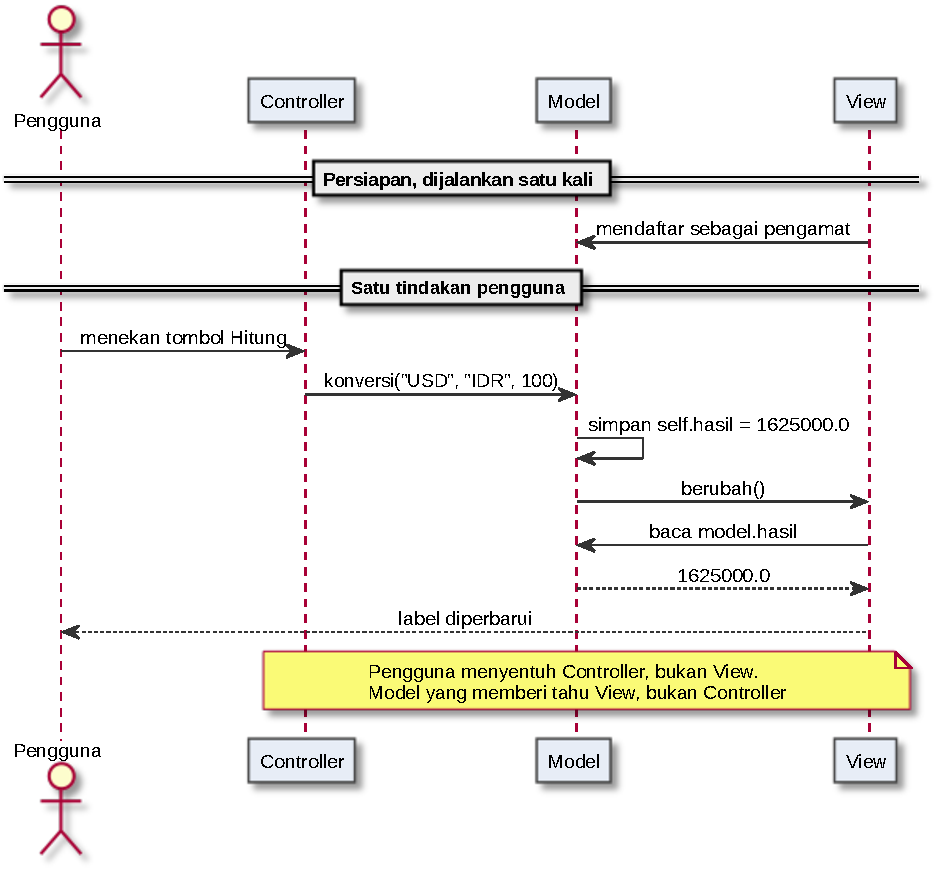
\includegraphics[width=0.95\textwidth]{sekuens-mvc-klasik.pdf}
  \caption{Diagram sekuens MVC klasik. Model yang memicu penggambaran, dan
    Controller tidak menyentuh View sama sekali}
  \label{fig:sekuens-mvc-klasik}
\end{figure}

Langkah keempat memuat perbedaan yang paling menentukan. Yang memicu
penggambaran adalah Model, bukan Controller. Controller bahkan tidak mengetahui
bahwa View sudah menggambar ulang. Susunan seperti itu memungkinkan satu Model
diamati banyak View sekaligus, dan seluruhnya diperbarui oleh satu pemberitahuan.

Bentuk kedua muncul karena kerangka kerja web bekerja dengan cara yang berbeda.
Permintaan datang, dilayani, lalu selesai, sehingga tidak ada View yang menetap
untuk diberi tahu. Gambar~\ref{fig:mvc-modern} menunjukkan bentuk tersebut.

Letak pengguna pada bentuk kedua berbeda dari bentuk klasiknya, dan perbedaan
itu sering terlewat. Pada bentuk klasik, Controller menafsirkan sendiri
peristiwa tetikus dan papan ketik, sehingga pengguna berhadapan langsung
dengannya. Pada bentuk masa kini, Controller tidak punya permukaan yang dapat
disentuh sama sekali.

Yang disentuh pengguna adalah View. Pada aplikasi web, pengguna menekan tautan
pada halaman yang sudah tergambar, lalu perute mengubahnya menjadi permintaan
dan mengantarkannya ke Controller. Pada aplikasi desktop, widget dimiliki View,
dan penangan widget itulah yang memanggil Controller. Keduanya berbeda pada
perantaranya, tetapi sama pada intinya, yaitu pengguna menyentuh View sedangkan
Controller hanya menerima permintaan yang sudah diteruskan.

\begin{figure}[htbp]
  \centering
  \begin{tikzpicture}[
    kotak/.style={draw, rounded corners=2pt, minimum width=2.1cm,
      minimum height=0.7cm, align=center, font=\scriptsize\bfseries},
    panah/.style={-{Stealth[length=1.8mm]}, thick}
  ]
    \node[kotak, fill=cPenghubung] (c) at (0,0) {Controller};
    \node[kotak, fill=cView] (v) at (0,-1.6) {View};
    \node[kotak, fill=cModel] (m) at (0,-3.2) {Model};
    \node[kotak, fill=cPengguna] (u) at (-3.7,-1.6) {Pengguna};
    % Pengguna dan View saling berhadapan.
    \draw[panah] ([yshift=1.6mm]u.east) -- ([yshift=1.6mm]v.west)
      node[midway, above, font=\tiny] {menekan};
    \draw[panah] ([yshift=-1.6mm]v.west) -- ([yshift=-1.6mm]u.east)
      node[midway, below, font=\tiny] {tampilan};
    % View meneruskan ke atas, Controller memerintah ke bawah.
    \draw[panah] ([xshift=-5mm]v.north) -- ([xshift=-5mm]c.south)
      node[midway, left, font=\tiny] {meneruskan};
    \draw[panah] ([xshift=5mm]c.south) -- ([xshift=5mm]v.north)
      node[midway, right, font=\tiny] {memerintah};
    % Controller menyerahkan rujukan Model, lalu View membaca hasilnya.
    \draw[panah] ([xshift=-5mm]v.south) -- ([xshift=-5mm]m.north)
      node[midway, left, font=\tiny] {membaca hasil};
    \draw[panah] (c.east) -- ++(1.7,0) |- (m.east)
      node[pos=0.22, right, font=\tiny] {memanggil};
  \end{tikzpicture}
  \caption{MVC pada kerangka kerja masa kini. Pengguna menyentuh View, lalu
    permintaannya diteruskan ke Controller. Controller memanggil Model, lalu
    memerintah View. View membaca hasil dari Model yang rujukannya sudah
    diserahkan Controller, dan Model tidak memberi tahu siapa pun}
  \label{fig:mvc-modern}
\end{figure}

Tabel~\ref{tab:dua-mvc} merangkum perbedaan keduanya.

\begin{table}[htbp]
  \centering
  \caption{Perbedaan MVC klasik dan MVC pada kerangka kerja masa kini}
  \label{tab:dua-mvc}
  \begin{tabularx}{\textwidth}{|l|X|X|}
    \hline
    \textbf{Hal} & \textbf{MVC klasik} & \textbf{MVC masa kini} \\
    \hline
    Pemicu penggambaran & Model memberi tahu View & Controller memerintah View \\
    \hline
    Sifat & Menetap, View hidup terus & Sekali jalan, permintaan lalu selesai \\
    \hline
    Peran Controller & Menangani masukan saja & Menangani masukan dan mengatur alur \\
    \hline
    Yang disentuh pengguna & Controller, sebab Controller menafsirkan tetikus dan papan ketik & View, lalu diteruskan ke Controller \\
    \hline
    Pengetahuan Model & Tahu ada yang mengamati & Tidak tahu apa pun \\
    \hline
  \end{tabularx}
\end{table}

Contoh pada bab ini memakai bentuk masa kini, sebab bentuk itulah yang paling
sering ditemui. Ciri khasnya terletak pada konstruktor View, yang menerima Model
sebagai argumen. Karena itu View tidak dapat dibuat tanpa Model, dan pengujian
logika tampilan tetap menuntut kedua objek tersebut ada. Tombolnya pun dimiliki
View, sehingga pengguna menyentuh View lalu View meneruskannya ke Controller.

\begin{lstlisting}[style=PythonStyle, caption={View pada MVC mengenal Model,
  sekaligus meneruskan tindakan pengguna, tersedia di
  \berkas{sources/chapter03/mvc.py}}, label=lst:mvc]
class View:

  def __init__(self, induk, model):
    self.model = model
    self.controller = None
    self.tombol = tk.Button(induk, text="Hitung",
                            command=self.saat_ditekan)

  def saat_ditekan(self):
    # Widget dimiliki View, sehingga pengguna menyentuh View.
    self.controller.tangani_masukan("USD", "IDR", 100)
\end{lstlisting}

Penelusuran satu permintaan memperjelas apa yang menyeberang antar komponen.
Pengguna memasukkan 100 USD ke IDR, lalu urutannya sebagai berikut.

\begin{enumerate}
  \item Pengguna menekan tombol milik View, lalu View memanggil
    \texttt{controller.tangani\_masukan} dengan tiga nilai mentah, yaitu
    \texttt{"USD"}, \texttt{"IDR"}, dan \texttt{100}.
  \item Controller memanggil \texttt{model.konversi} dengan ketiga nilai
    tersebut.
  \item Model menghitung, lalu \textbf{menyimpan hasilnya di dalam dirinya
    sendiri} sebagai \texttt{self.hasil}.
  \item Controller memanggil \texttt{view.render} tanpa membawa data apa pun.
  \item View \textbf{menarik sendiri} nilai \texttt{model.hasil}, lalu menyusun
    teks \texttt{Hasil: 1,625,000.00}.
\end{enumerate}

Gambar~\ref{fig:sekuens-mvc} menunjukkan urutan tersebut sebagai diagram
sekuens.

\begin{figure}[htbp]
  \centering
  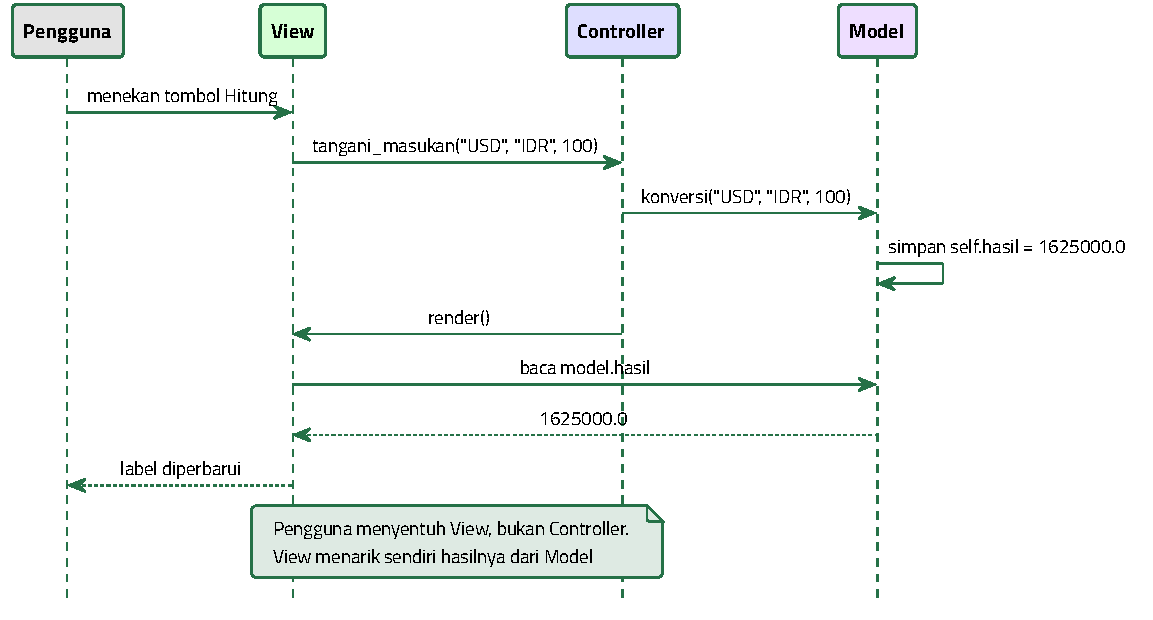
\includegraphics[width=0.95\textwidth]{sekuens-mvc.pdf}
  \caption{Diagram sekuens MVC. Hasil disimpan di Model, lalu ditarik sendiri oleh View}
  \label{fig:sekuens-mvc}
\end{figure}

Ciri khas MVC terletak pada langkah kelima. Hasil tidak dikirimkan kepada View,
melainkan diambil View dari Model. Karena itu View wajib mengenal Model.

Perlu satu penegasan agar tidak salah paham. View memang membaca Model, tetapi
View tidak mencari sendiri Model yang mana. Rujukannya diserahkan lebih dahulu,
yaitu lewat konstruktor pada aplikasi desktop atau lewat objek yang dititipkan
Controller pada aplikasi web. Jadi Controller tetap memegang kendali alurnya,
sedangkan View hanya membaca isi objek yang sudah diberikan kepadanya.

\subsection{Model-View-Presenter}

MVP diperkenalkan Potel~\cite{potel1996mvp} sebagai penyederhanaan MVC. MVP
menjadikan View pasif. Presenter mengerjakan seluruh penyusunan teks, lalu
mendorong hasilnya ke View. Gambar~\ref{fig:mvp} menunjukkan bahwa tidak ada
panah dari View ke Model. Ruang di bawah View kosong, dan kekosongan itulah
pembeda MVP dari MVC.

\begin{figure}[htbp]
  \centering
  \begin{tikzpicture}[
    kotak/.style={draw, rounded corners=2pt, minimum width=2.1cm,
      minimum height=0.7cm, align=center, font=\scriptsize\bfseries},
    panah/.style={-{Stealth[length=1.8mm]}, thick}
  ]
    \node[kotak, fill=cPenghubung] (p) at (0,0) {Presenter};
    \node[kotak, fill=cView] (v) at (0,-1.6) {View};
    \node[kotak, fill=cModel] (m) at (0,-3.2) {Model};
    \node[kotak, fill=cPengguna] (u) at (-3.7,-1.6) {Pengguna};
    % Pengguna hanya berhadapan dengan View, tidak dengan Presenter.
    \draw[panah] ([yshift=1.6mm]u.east) -- ([yshift=1.6mm]v.west)
      node[midway, above, font=\tiny] {menyentuh};
    \draw[panah] ([yshift=-1.6mm]v.west) -- ([yshift=-1.6mm]u.east)
      node[midway, below, font=\tiny] {tampilan};
    % View meneruskan ke atas, Presenter mendorong teks ke bawah.
    \draw[panah] ([xshift=-5mm]v.north) -- ([xshift=-5mm]p.south)
      node[midway, left, font=\tiny] {meneruskan};
    \draw[panah] ([xshift=5mm]p.south) -- ([xshift=5mm]v.north)
      node[midway, right, font=\tiny] {mendorong teks};
    % Tidak ada panah dari View ke Model. Itulah inti passive view.
    \draw[panah] (p.east) -- ++(1.7,0) |- (m.east)
      node[pos=0.22, right, font=\tiny] {memanggil};
  \end{tikzpicture}
  \caption{MVP, dengan View pasif yang tidak mengenal Model. Pengguna tetap
    menyentuh View, lalu View meneruskannya ke Presenter}
  \label{fig:mvp}
\end{figure}

View pada MVP hanya menyimpan teks yang diterimanya. Karena tidak ada perilaku
yang perlu ditiru selain menyimpan, View tersebut dapat diganti tiruan sederhana
saat diuji.

Bentuk yang dipakai di sini disebut \textit{passive view}, yaitu View yang sama
sekali tidak mengenal komponen lain. Banyak penerapan MVP memakai bentuk lain,
yaitu View menyimpan rujukan ke Presenter agar dapat meneruskan tindakan
pengguna. Pada bentuk tersebut hubungannya menjadi dua arah, dan angka
ketergantungannya bertambah satu.

\begin{lstlisting}[style=PythonStyle, caption={View pasif pada MVP, tersedia di
  \berkas{sources/chapter03/mvp.py}}, label=lst:mvp]
class View:
  """Menyimpan teks yang diberikan Presenter, tanpa logika apa pun."""

  def tampilkan(self, teks):
    self.teks = teks
\end{lstlisting}

Penelusuran permintaan yang sama pada MVP berbeda mulai langkah ketiga.

\begin{enumerate}
  \item Presenter menerima tiga nilai mentah.
  \item Presenter memanggil \texttt{model.konversi}, dan Model
    \textbf{mengembalikan} angka \texttt{1625000.0} sebagai nilai balik.
  \item Presenter menyusun teks \texttt{Hasil: 1,625,000.00}.
  \item Presenter memanggil \texttt{view.tampilkan} dengan \textbf{membawa teks
    yang sudah jadi}.
  \item View menyimpan teks tersebut tanpa mengolahnya.
\end{enumerate}

Gambar~\ref{fig:sekuens-mvp} menunjukkan urutan tersebut sebagai diagram
sekuens.

\begin{figure}[htbp]
  \centering
  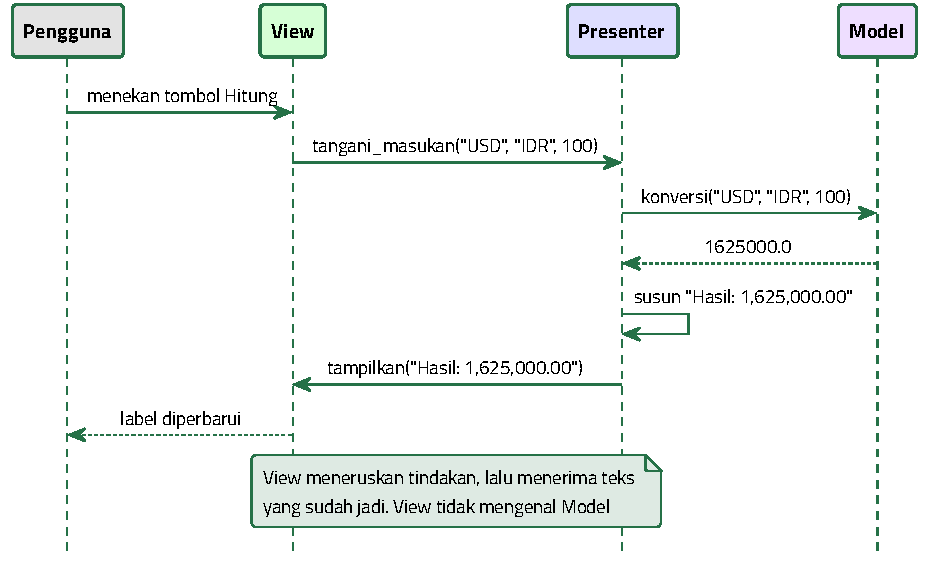
\includegraphics[width=0.95\textwidth]{sekuens-mvp.pdf}
  \caption{Diagram sekuens MVP. Teks yang sudah jadi didorong Presenter ke View}
  \label{fig:sekuens-mvp}
\end{figure}

Perbedaannya jelas. Pada MVC hasil disimpan di Model lalu ditarik View,
sedangkan pada MVP hasil dikembalikan ke Presenter lalu didorong ke View. View
karena itu tidak perlu mengenal Model.

\subsection{Model-View-ViewModel}

MVVM diperkenalkan Gossman~\cite{gossman2005mvvm} bersama kerangka kerja
Windows Presentation Foundation. MVVM membalik arah pemberitahuan. ViewModel
menyediakan properti yang dapat
diamati, lalu View mendaftarkan diri sebagai pengamat. Ketika properti berubah,
View memperbarui dirinya sendiri. Gambar~\ref{fig:mvvm} menunjukkan bahwa
ViewModel tidak mengenal View.

\begin{figure}[htbp]
  \centering
  \begin{tikzpicture}[
    kotak/.style={draw, rounded corners=2pt, minimum width=2.1cm,
      minimum height=0.7cm, align=center, font=\scriptsize\bfseries},
    panah/.style={-{Stealth[length=1.8mm]}, thick}
  ]
    \node[kotak, fill=cModel] (m) {Model};
    \node[kotak, fill=cPenghubung, below=0.6cm of m] (vm) {ViewModel};
    \node[kotak, fill=cView, below=0.6cm of vm] (v) {View};
    \node[kotak, fill=cPengguna, left=1.5cm of v] (u) {Pengguna};
    \draw[panah] (vm) -- node[right, font=\tiny] {memanggil} (m);
    \draw[panah] (v) -- node[right, font=\tiny] {mengamati} (vm);
    \draw[panah] (u) -- node[above, font=\tiny] {menyentuh} (v);
  \end{tikzpicture}
  \caption{MVVM, dengan View yang mengamati properti milik ViewModel}
  \label{fig:mvvm}
\end{figure}

Jumlah ketergantungan MVVM sama dengan MVC, yaitu tiga. Arahnya yang berbeda.
Pada MVC View mengenal Model, sedangkan pada MVVM View mengenal ViewModel dan
ViewModel tidak mengenal View. Karena itu logika tampilan dapat diuji cukup
dengan membaca properti, tanpa membuat objek View.

\begin{lstlisting}[style=PythonStyle, caption={View mengikat diri pada properti,
  tersedia di \berkas{sources/chapter03/mvvm.py}}, label=lst:mvvm]
class View:
  """Mengikat diri pada properti ViewModel dan menyimpan nilai terbarunya."""

  def __init__(self, view_model):
    self.terakhir = None
    view_model.teks.amati(self.saat_berubah)
\end{lstlisting}

Penelusuran permintaan yang sama pada MVVM berbeda pada arah pemberitahuannya.

\begin{enumerate}
  \item ViewModel menerima tiga nilai mentah.
  \item ViewModel memanggil \texttt{model.konversi} dan menerima
    \texttt{1625000.0}.
  \item ViewModel menulis teks ke propertinya lewat \texttt{teks.ubah}.
  \item Properti tersebut \textbf{memanggil seluruh pengamatnya} satu per satu.
  \item View menerima teks baru lewat \texttt{saat\_berubah}, lalu memperbarui
    dirinya.
\end{enumerate}

Gambar~\ref{fig:sekuens-mvvm} menunjukkan urutan tersebut sebagai diagram
sekuens. Perhatikan langkah pertama, yaitu View mendaftarkan diri sebagai
pengamat sebelum permintaan datang.

\begin{figure}[htbp]
  \centering
  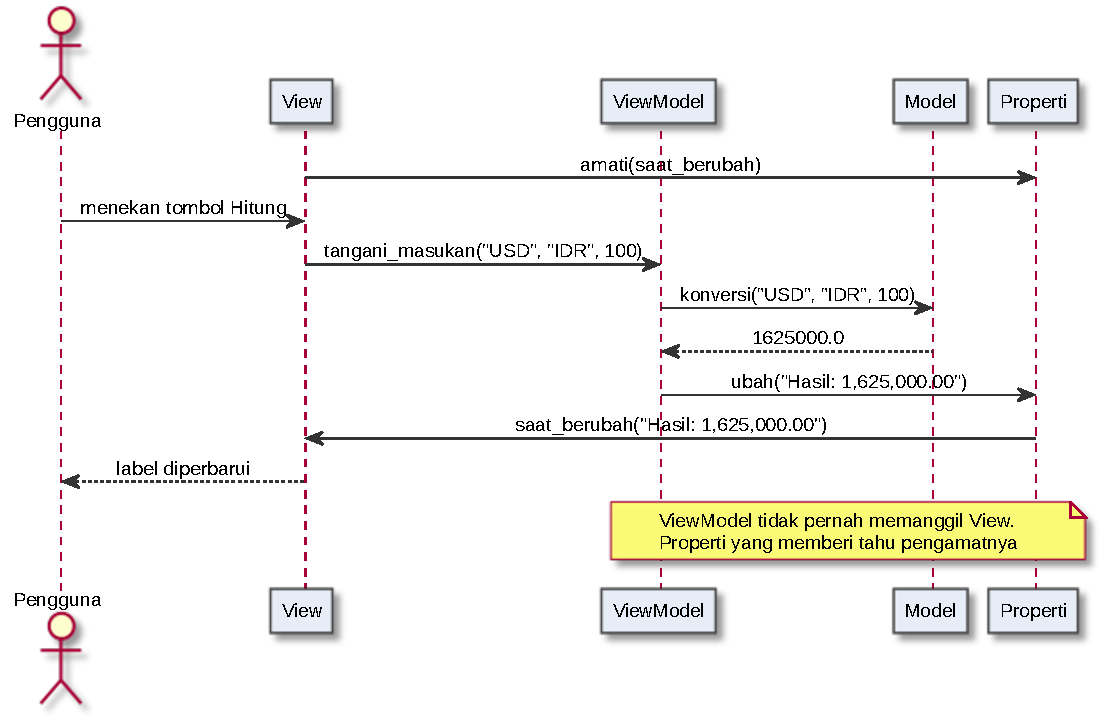
\includegraphics[width=0.95\textwidth]{sekuens-mvvm.pdf}
  \caption{Diagram sekuens MVVM. Properti yang memberi tahu pengamatnya, bukan ViewModel}
  \label{fig:sekuens-mvvm}
\end{figure}

ViewModel tidak pernah memanggil View. ViewModel hanya mengubah nilai properti,
dan properti itulah yang memberi tahu siapa pun yang mendaftar. Karena itu satu
properti dapat diamati beberapa View sekaligus tanpa ViewModel mengetahuinya.

\subsection{Model-View-Intent}

MVI menghapus kelas penghubung sama sekali. Setiap tindakan pengguna dibungkus
menjadi Intent, lalu sebuah fungsi reduksi mengubah pasangan keadaan lama dan
Intent menjadi keadaan baru yang tidak dapat diubah lagi.
Gambar~\ref{fig:mvi} menunjukkan susunannya.

\begin{figure}[htbp]
  \centering
  \begin{tikzpicture}[
    kotak/.style={draw, rounded corners=2pt, minimum width=1.9cm,
      minimum height=0.7cm, align=center, font=\scriptsize\bfseries},
    panah/.style={-{Stealth[length=1.8mm]}, thick}
  ]
    \node[kotak, fill=cPenghubung] (i) {Intent};
    \node[kotak, fill=cPenghubung, right=1.0cm of i] (r) {reduksi()};
    \node[kotak, fill=cModel, right=1.0cm of r] (k) {Keadaan};
    \node[kotak, fill=cView, right=1.0cm of k] (v) {View};
    \node[kotak, fill=cPengguna, above=0.5cm of v] (u) {Pengguna};
    \draw[panah] (i) -- (r);
    \draw[panah] (r) -- (k);
    \draw[panah] (k) -- (v);
    \draw[panah] (u) -- node[right, font=\tiny] {menyentuh} (v);
    \draw[panah] (v.south) -- ++(0,-0.8) -| (i.south)
      node[pos=0.25, below, font=\tiny] {dibungkus menjadi Intent};
  \end{tikzpicture}
  \caption{MVI bersifat searah dan membentuk siklus. View menggambar Keadaan,
    lalu tindakan pengguna kembali menjadi Intent}
  \label{fig:mvi}
\end{figure}

Listing~\ref{lst:reduksi} memperlihatkan fungsi tersebut. Karena fungsi itu
murni, seluruh keadaan yang pernah digambar dapat disimpan lalu diputar ulang
persis seperti semula. Sifat itu membuat antarmuka yang keluarannya
berubah-ubah tetap dapat diuji secara pasti.

\begin{lstlisting}[style=PythonStyle, caption={Fungsi reduksi pada MVI,
  tersedia di \berkas{sources/chapter03/mvi.py}}, label=lst:reduksi]
def reduksi(keadaan, intent):
  """Mengubah keadaan lama dan sebuah Intent menjadi keadaan baru.

  Fungsi ini murni, artinya keluarannya hanya bergantung pada kedua masukannya.
  Sifat itulah yang membuat riwayat tampilan dapat diputar ulang.
  """
  try:
    hasil = domain.hitung_konversi(intent.kode_asal, intent.kode_tujuan,
                                   intent.nominal)
    return replace(keadaan, teks=f"Hasil: {hasil:,.2f}", sedang_sibuk=False)
  except (ValueError, LookupError) as kesalahan:
    return replace(keadaan, teks=f"Galat: {kesalahan}", sedang_sibuk=False)
\end{lstlisting}

Agar keempat varian tidak berhenti sebagai nama, Tabel~\ref{tab:contoh-mv}
menunjukkan isi setiap peran pada aplikasi konversi yang dipakai sepanjang bab
ini. Perhatikan bahwa isi Model dan View hampir sama pada keempatnya, sedangkan
peran penghubungnya berbeda jauh.

\begin{table}[htbp]
  \centering
  \caption{Contoh isi setiap peran pada aplikasi konversi}
  \label{tab:contoh-mv}
  \begin{tabularx}{\textwidth}{|l|X|X|}
    \hline
    \textbf{Varian} & \textbf{Isi penghubungnya} & \textbf{Yang dilakukan View} \\
    \hline
    MVC & Controller meneruskan masukan ke Model & Membaca Model lalu menyusun teks \\
    \hline
    MVP & Presenter menyusun teks lalu mendorongnya & Menyimpan teks yang diterima \\
    \hline
    MVVM & ViewModel menulis hasil ke properti & Memperbarui diri saat properti berubah \\
    \hline
    MVI & Fungsi reduksi menghasilkan keadaan baru & Menggambar keadaan yang diterima \\
    \hline
  \end{tabularx}
\end{table}

Kasus berikut memperlihatkan akibatnya pada pekerjaan sehari-hari. Sebuah tim
ingin menguji aturan penolakan nominal nol. Pada MVC, pengujian tersebut tetap
menuntut objek View dibuat lebih dahulu, sebab Controller merujuk View. View
menuntut Model, dan Model menuntut sambungan data. Pengujian yang seharusnya
memeriksa satu aturan akhirnya menyalakan hampir seluruh aplikasi. Pada MVI,
pengujian yang sama cukup memanggil satu fungsi reduksi tanpa membuat objek apa
pun.

Yang menentukan bukan jumlah kelasnya, melainkan komponen apa yang dituntut
View. Itulah sebabnya perbandingan pada bab ini memakai ketergantungan sebagai
ukuran, bukan panjang kode.

Penelusuran permintaan yang sama pada MVI tidak memakai pemanggilan metode
antar objek sama sekali.

\begin{enumerate}
  \item Tindakan pengguna dibungkus menjadi
    \texttt{IntentKonversi("USD", "IDR", 100)}.
  \item Fungsi \texttt{reduksi} dipanggil dengan dua masukan, yaitu keadaan lama
    dan Intent tersebut.
  \item Di dalamnya \texttt{domain.hitung\_konversi} menghasilkan
    \texttt{1625000.0}.
  \item Fungsi tersebut \textbf{mengembalikan objek Keadaan baru} berisi teks
    hasil, tanpa mengubah keadaan lama.
  \item View menggambar Keadaan tersebut, lalu menyimpannya ke dalam riwayat.
\end{enumerate}

Gambar~\ref{fig:sekuens-mvi} menunjukkan urutan tersebut sebagai diagram
sekuens.

\begin{figure}[htbp]
  \centering
  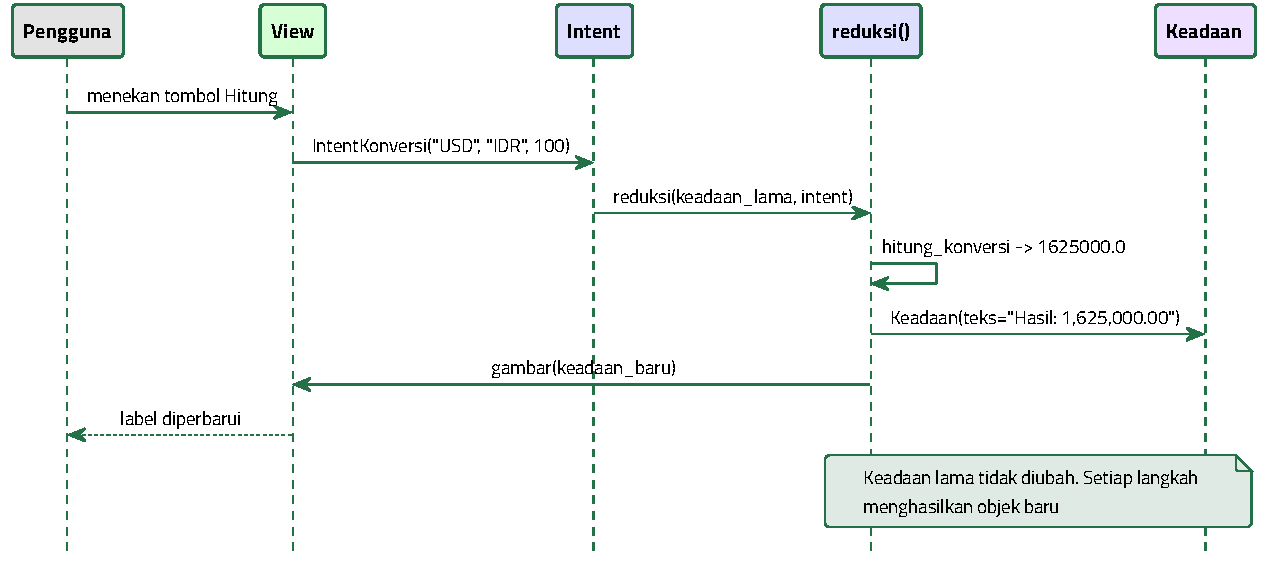
\includegraphics[width=0.95\textwidth]{sekuens-mvi.pdf}
  \caption{Diagram sekuens MVI. Setiap langkah menghasilkan objek baru, tanpa mengubah yang lama}
  \label{fig:sekuens-mvi}
\end{figure}

Seluruh isi tampilan terbungkus dalam satu objek Keadaan. Karena keadaan lama
tidak pernah diubah, seluruh riwayat tersimpan utuh dan dapat diputar ulang.

Tabel~\ref{tab:aliran-data} merangkum apa yang menyeberang menuju View pada
keempat varian.

\begin{table}[htbp]
  \centering
  \caption{Apa yang menyeberang menuju View pada keempat varian}
  \label{tab:aliran-data}
  \begin{tabularx}{\textwidth}{|l|X|X|}
    \hline
    \textbf{Varian} & \textbf{Yang diterima View} & \textbf{Cara View memperolehnya} \\
    \hline
    MVC & Tidak ada, hanya perintah menggambar & Menarik sendiri dari Model \\
    \hline
    MVP & Teks yang sudah jadi & Didorong Presenter lewat pemanggilan metode \\
    \hline
    MVVM & Nilai properti yang baru & Diberi tahu properti yang diamatinya \\
    \hline
    MVI & Satu objek Keadaan yang utuh & Diserahkan sebagai argumen saat digambar \\
    \hline
  \end{tabularx}
\end{table}

\section{Produk yang Memakai Setiap Varian}

Keempat varian tersebut bukan bahan kuliah semata. Setiap varian punya kerangka
kerja atau produk yang memakainya. Tabel~\ref{tab:produk-mv} merangkum contoh
yang paling sering ditemui.

\begin{table}[htbp]
  \centering
  \caption{Contoh produk dan kerangka kerja untuk setiap varian}
  \label{tab:produk-mv}
  \begin{tabularx}{\textwidth}{|l|X|X|}
    \hline
    \textbf{Varian} & \textbf{Contoh produk} & \textbf{Catatan} \\
    \hline
    MVC klasik & Smalltalk-80 & Bentuk aslinya, dengan Model yang memberi tahu View \\
    \hline
    MVC masa kini & Ruby on Rails, Laravel, Spring MVC, ASP.NET Core MVC & Controller menerima permintaan dari perute, lalu memerintah View \\
    \hline
    MVP & Google Web Toolkit, Windows Forms, aplikasi Android sebelum era Jetpack & Presenter mendorong teks jadi ke View yang pasif \\
    \hline
    MVVM & Windows Presentation Foundation, .NET MAUI, Vue.js versi awal & View mengamati properti pada ViewModel \\
    \hline
    MVI & Redux, arsitektur Elm, Flutter Bloc & Keadaan diganti utuh oleh fungsi reduksi. Android menganjurkan aliran searah dengan nama UDF, tanpa memakai istilah MVI \\
    \hline
  \end{tabularx}
\end{table}

Empat hal perlu penjelasan tambahan, sebab keempatnya sering menimbulkan salah paham.

\textbf{Django tidak memakai penamaan MVC.} Django menyebut polanya
\textit{Model-Template-View} atau MTV. Berkas yang disebut \texttt{views.py} pada
Django sebenarnya berperan sebagai Controller, sebab berkas tersebut memilih
data mana yang disajikan. Templat Django itulah yang berperan sebagai View.
Dokumentasi resminya menyatakan Controller pada Django adalah kerangka kerjanya
sendiri, yaitu bagian yang mengantar permintaan ke fungsi yang
tepat~\cite{django2026faq}.

\textbf{Android tidak menyebut dirinya MVVM.} Banyak tulisan menyebut Android
memakai MVVM karena ada kelas bernama \texttt{ViewModel}. Dokumentasi resminya
tidak memakai istilah tersebut sama sekali. Dokumentasi tersebut menyebut
\texttt{ViewModel} sebagai \textit{state holder}, yaitu pemegang keadaan layar,
di dalam susunan berlapis yang terdiri atas lapisan antarmuka, domain, dan
data~\cite{android2026viewmodel}. Kemiripannya dengan MVVM memang ada, sebab
View mengamati keadaan dan \texttt{ViewModel} tidak mengenal View. Meskipun
begitu, penyebutannya sebaiknya tetap hati-hati.

\textbf{Intent pada Android dan Intent pada MVI memakai gagasan yang sama.}
Kesamaan namanya bukan kebetulan. Keduanya membungkus niat menjadi objek data,
lalu menyerahkan objek tersebut kepada pihak yang menyalurkannya.

Intent untuk mengirim pesan singkat memperjelas hal tersebut. Objek tersebut
tidak mengirim apa pun sendiri. Objek tersebut hanya menyatakan adanya niat
mengirim pesan ke nomor tertentu. Sistem operasi lalu memilih aplikasi mana yang
mengerjakannya, dan pengguna bahkan dapat ikut memilih ketika aplikasinya lebih
dari satu. Dokumentasi Android menyebutnya objek pesan untuk meminta tindakan
dari komponen aplikasi lain~\cite{android2026intent}. Intent pada MVI bekerja
dengan cara yang sama, hanya saja penyalurnya berupa fungsi reduksi.

Tujuan keduanya pun sama. Sebuah Intent dikirim agar ada keadaan yang berubah,
atau agar ada proses tertentu yang dijalankan. Objek itu sendiri tidak
mengerjakan apa pun.

Gagasan tersebut dikenal luas dengan nama \textit{command}. Sebuah
\textit{command} adalah permintaan agar sistem melakukan tindakan yang mengubah
keadaannya. Wujudnya berupa kelas yang hanya berisi data yang diperlukan,
semacam \textit{Data Transfer Object} khusus~\cite{microsoft2021command}.
Rumusan tersebut berlaku untuk keduanya tanpa perubahan sedikit pun. Akibat yang
menyertainya juga sama. Pengirim tidak perlu mengenal pihak yang mengerjakan,
permintaannya dapat dicatat dan diperiksa, dan pengerjanya dapat diganti tanpa
menyentuh pengirimnya.

Yang berbeda hanyalah tingkat penerapannya, bukan gagasan maupun tujuannya.
Dua baris pertama pada Tabel~\ref{tab:dua-intent} karena itu berisi hal yang
persis sama untuk kedua kolomnya.

\begin{table}[htbp]
  \centering
  \caption{Intent pada Android dan Intent pada MVI, satu gagasan pada dua
    tingkat penerapan}
  \label{tab:dua-intent}
  \begin{tabularx}{\textwidth}{|l|X|X|}
    \hline
    \textbf{Hal} & \textbf{Intent pada Android} & \textbf{Intent pada MVI} \\
    \hline
    Gagasannya & Niat dibungkus menjadi objek data & Niat dibungkus menjadi objek data \\
    \hline
    Tujuannya & Ada keadaan yang berubah atau proses yang dijalankan & Ada keadaan yang berubah atau proses yang dijalankan \\
    \hline
    Contohnya & Niat mengirim pesan singkat ke satu nomor & Niat mengonversi 100 USD menjadi IDR \\
    \hline
    Penyalurnya & Sistem operasi Android & Fungsi reduksi \\
    \hline
    Cakupannya & Melintasi komponen dan aplikasi & Berada di dalam satu layar \\
    \hline
    Wujud perubahannya & Komponen lain dijalankan, misalnya aplikasi pesan terbuka & Objek keadaan baru dikembalikan \\
    \hline
  \end{tabularx}
\end{table}

Kesimpulannya perlu ditarik hati-hati. Pemakaian kelas \texttt{Intent} tidak
dengan sendirinya menjadikan sebuah aplikasi Android memakai MVI. MVI menuntut
lebih dari sekadar membungkus niat, yaitu keadaan layar yang diganti utuh oleh
fungsi reduksi. Bagian Android yang benar-benar sejajar dengan MVI justru
terletak di tempat lain. Dokumentasi Android menganjurkan
\textit{unidirectional data flow} atau UDF, yaitu aliran data satu arah.
Keadaan mengalir turun menuju antarmuka, sedangkan peristiwa mengalir naik
menuju \texttt{ViewModel}~\cite{android2026uilayer}. Bentuk aliran tersebut sama
dengan MVI, meskipun istilah MVI tidak dipakai dalam dokumentasinya.

\textbf{Redux mewarisi arsitektur Elm.} Dokumentasi Redux menyebut Elm sebagai
sumber gagasannya. Elm memakai susunan \textit{model view update}, dan fungsi
pembaruannya bertanda tangan \texttt{(action, state) => state}. Fungsi tersebut
sama perannya dengan fungsi reduksi pada Redux~\cite{redux2026priorart}. Karena
itu Redux menjadi contoh MVI yang paling mudah ditemui.

Vue.js pada dokumentasi versi awalnya menyebut setiap instansnya sebagai
ViewModel, dan karena itu variabelnya dinamai \texttt{vm}~\cite{vue2016instance}.
Dokumentasi versi terbarunya tidak lagi memakai istilah tersebut. Penyebutan
seperti ini memang berubah seiring waktu, sehingga rujukan versi perlu ikut
dicatat.

\section{Ketergantungan View sebagai Pembeda}

Satu pertanyaan cukup untuk membedakan keempat varian, yaitu komponen apa yang
dikenal oleh View. Jawabannya menentukan seberapa mudah logika tampilan diuji
tanpa menjalankan antarmuka sungguhan.

Analogi yang mendekati adalah loket informasi di kampus. Petugas loket yang
harus membuka lemari arsip sendiri sulit digantikan, sebab penggantinya harus
mengenal isi lemari tersebut. Petugas yang hanya membacakan lembar yang sudah
disiapkan bagian lain mudah digantikan siapa pun. View pada MVP dan MVI berperan
seperti petugas kedua.

Tabel~\ref{tab:ketergantungan-mv} merangkum hasil pemeriksaan nyata memakai
\texttt{periksa\_mv.py}. Kolom terakhir menunjukkan cara pengujian yang paling
sedikit menyentuh antarmuka.

\begin{table}[htbp]
  \centering
  \caption{Ketergantungan dan cara pengujian keempat varian}
  \label{tab:ketergantungan-mv}
  \begin{tabularx}{\textwidth}{|l|l|l|X|}
    \hline
    \textbf{Varian} & \textbf{Total} & \textbf{View butuh} & \textbf{Cara pengujian} \\
    \hline
    MVC & 3 & Model & Membutuhkan View asli \\
    \hline
    MVP & 2 & tidak ada & Cukup View tiruan \\
    \hline
    MVVM & 3 & ViewModel & Tanpa View, cukup membaca propertinya \\
    \hline
    MVI & 0 & tidak ada & Tanpa View, cukup memanggil fungsi reduksi \\
    \hline
  \end{tabularx}
\end{table}

Angka pada tabel tersebut punya dua bacaan. Pertama, MVI mencatat nol
ketergantungan karena penghubungnya berupa fungsi, bukan kelas yang menyimpan
rujukan ke komponen lain. Kedua, MVVM mencatat total yang sama dengan MVC,
tetapi ketergantungannya menunjuk ke arah yang berbeda. Pada MVC, View mengenal
Model. Pada MVVM, View mengenal ViewModel, sedangkan ViewModel tidak mengenal
View. Jumlah yang sama karena itu tidak berarti sifatnya sama.

\section{Ketika Satu Komponen Menggemuk}

Pemisahan peran hanya bertahan bila setiap komponen menolak pekerjaan yang bukan
miliknya. Bila penolakan itu tidak terjadi, satu komponen menampung hampir semua
kode. Komponen lain tinggal menjadi hiasan. Keadaan tersebut punya nama sendiri,
dan namanya diambil dari komponen yang menggemuk.

\subsection{Fat Controller}

\textit{Fat controller} adalah Controller yang menyimpan aturan bisnis. Nasihat
resminya sederhana. Controller bertugas menerima permintaan, memanggil pihak
yang mengerjakan, lalu menyiapkan balasan~\cite{rails2026controller}. Aturan
bisnisnya bukan miliknya.

Listing~\ref{lst:fat-controller} memperlihatkan bentuk yang keliru. Validasi,
perhitungan, dan penyusunan teks menumpuk di satu tempat.

\begin{lstlisting}[style=PythonStyle, caption={Controller yang menggemuk, sebab
  aturan bisnisnya ikut ditulis di dalamnya}, label=lst:fat-controller]
class Controller:

  def tangani_masukan(self, asal, tujuan, nominal):
    if nominal <= 0:                      # aturan bisnis
      return "Galat: nominal harus positif"
    if nominal > 1_000_000_000:           # aturan bisnis
      return "Galat: nominal melewati batas"
    kurs = self.model.cari_kurs(asal, tujuan)
    hasil = nominal * kurs                # perhitungan bisnis
    return f"Hasil: {hasil:,.2f}"         # penyusunan tampilan
\end{lstlisting}

Akibatnya ada tiga. Pertama, aturan tersebut tidak dapat dipakai ulang. Pintu
masuk lain seperti antarmuka baris perintah atau penjadwal harus menyalin ulang
aturan yang sama. Kedua, pengujiannya menuntut konteks permintaan, padahal yang
diuji hanyalah perkalian dan perbandingan angka. Ketiga, aturan yang sama
tersebar di banyak Controller, sehingga satu perubahan kebijakan menuntut
penyuntingan di banyak tempat.

Perbaikannya adalah memindahkan kedua pemeriksaan dan perkaliannya ke Model,
lalu menyisakan pemanggilan saja di Controller. Bab~\ref{bab:lapisan} sudah
memakai pola tersebut pada \texttt{hitung\_konversi}.

Pada pemrograman aplikasi iOS, gejala yang sama dikenal dengan plesetan
\textit{Massive View Controller}. Singkatan MVC dibaca ulang karena View dan
Controller menyatu, lalu keduanya menampung seluruh kode.

\subsection{Fat Model}

\textit{Fat model} adalah kebalikannya. Nasihat \textit{skinny controller, fat
model} memang benar sebagai arah, tetapi sering dibaca berlebihan. Model lalu
menampung empat hal sekaligus, yaitu aturan bisnis, akses basis data, penyusunan
teks tampilan, dan pengiriman pemberitahuan.

Model seperti itu punya banyak alasan untuk berubah. Perubahan tata letak
kolom basis data menyentuhnya. Perubahan format tanggal menyentuhnya. Perubahan
kebijakan diskon juga menyentuhnya. Kelas dengan ribuan baris biasanya lahir
dari sini.

Perbaikannya bukan mengembalikan kode ke Controller. Perbaikannya adalah membagi
Model menjadi beberapa bagian, misalnya bagian aturan domain, bagian akses
penyimpanan, dan bagian penyusunan teks. Bab~\ref{bab:port} membahas pemisahan
tersebut lebih jauh memakai port dan adapter.

\subsection{Fat View}

\textit{Fat view} adalah View yang menyimpan logika. Gejalanya berupa
percabangan dan perhitungan di dalam templat. Contohnya penghitungan diskon,
penentuan peringkat, atau pemilihan pesan berdasarkan banyak syarat.

Kerugiannya jelas. Logika di dalam templat sulit diuji tanpa menggambar
antarmuka. Logika tersebut juga mudah tersalin ke templat lain, sebab menyalin
lebih cepat daripada memindahkannya ke tempat yang benar. MVP dan MVI menekan
gejala ini secara bawaan, sebab View pada kedua varian tersebut hanya menerima
hasil yang sudah jadi.

Tabel~\ref{tab:gemuk} merangkum ketiga gejala tersebut.

\begin{table}[htbp]
  \centering
  \caption{Gejala komponen yang menggemuk beserta perbaikannya}
  \label{tab:gemuk}
  \begin{tabularx}{\textwidth}{|l|X|X|}
    \hline
    \textbf{Gejala} & \textbf{Tanda yang terlihat} & \textbf{Perbaikan} \\
    \hline
    Fat controller & Validasi dan perhitungan ada di Controller & Pindahkan aturannya ke Model \\
    \hline
    Fat model & Satu kelas mengurus aturan, basis data, dan format & Bagi menjadi beberapa bagian menurut alasan berubahnya \\
    \hline
    Fat view & Percabangan dan perhitungan ada di templat & Susun teksnya di Presenter atau di fungsi reduksi \\
    \hline
  \end{tabularx}
\end{table}

Satu catatan penting menutup bagian ini. Alat \texttt{periksa\_mv.py} pada bab
ini mengukur arah ketergantungan, bukan ukuran komponennya. Sebuah program bisa
saja mencatat angka yang rapi, tetapi seluruh aturannya menumpuk di satu kelas.
Arah panah yang benar karena itu belum menjamin pembagian kerja yang sehat.
Jumlah baris dan jumlah method perlu ikut dilihat.

\section{Kelebihan dan Kekurangan}

Tabel~\ref{tab:untung-rugi-mv} merangkum untung rugi keempat varian tersebut.

\begin{table}[htbp]
  \centering
  \caption{Perbandingan keempat varian Model-View-*}
  \label{tab:untung-rugi-mv}
  \begin{tabularx}{\textwidth}{|l|X|X|}
    \hline
    \textbf{Varian} & \textbf{Kelebihan} & \textbf{Kekurangan} \\
    \hline
    MVC & Paling sederhana, banyak didukung framework & View mengenal Model, sehingga sulit diuji terpisah \\
    \hline
    MVP & View pasif dan mudah diganti tiruan & Presenter mudah membengkak karena memuat seluruh penyusunan teks \\
    \hline
    MVVM & Pembaruan tampilan berjalan otomatis lewat pengamatan & Membutuhkan mekanisme properti yang dapat diamati \\
    \hline
    MVI & Keadaan tetap, riwayat dapat diputar ulang & Setiap tindakan harus dibungkus menjadi Intent, sehingga kode bertambah \\
    \hline
  \end{tabularx}
\end{table}

Pemilihan varian jarang bebas sepenuhnya. Framework antarmuka biasanya sudah
menganjurkan satu varian tertentu, dan melawan anjuran tersebut berbiaya mahal.
Yang tetap dapat dipilih adalah seberapa banyak logika yang dititipkan ke View.
Semakin sedikit logika di dalam View, semakin besar bagian aplikasi yang dapat
diuji tanpa menjalankan antarmuka.

\section{Ringkasan}

Kelompok pola Model-View-* memisahkan tampilan dari aturan bisnis. Seluruh
varian membagi aplikasi menjadi bagian yang menyimpan data, bagian yang
menampilkan, dan bagian yang menghubungkan keduanya. Perbedaan antar varian
terletak pada cara bagian penghubung bekerja, bukan pada tujuannya.

Pembeda yang paling menentukan adalah komponen yang dikenal oleh View. Pada MVC
View mengenal Model, pada MVVM View mengenal ViewModel, sedangkan pada MVP dan
MVI View tidak mengenal apa pun. Semakin sedikit yang dikenal View, semakin
besar bagian aplikasi yang dapat diuji tanpa menjalankan antarmuka.

Pengukuran pada bab ini menunjukkan jumlah ketergantungan saja tidak cukup untuk
menilai sebuah varian. MVC dan MVVM sama-sama mencatat tiga ketergantungan,
tetapi arahnya berbeda, dan perbedaan arah itulah yang menentukan kemudahan
pengujiannya. Angka perlu dibaca bersama arahnya.

MVI mencatat nol ketergantungan karena penghubungnya berupa fungsi murni.
Sifat murni tersebut memberi keuntungan tambahan, yaitu seluruh keadaan yang
pernah digambar dapat disimpan lalu diputar ulang. Harganya, setiap tindakan
pengguna harus dibungkus menjadi Intent, sehingga jumlah kode bertambah.

Pemilihan varian pada praktiknya lebih sering ditentukan oleh framework yang
dipakai daripada oleh pertimbangan bebas. Yang tetap dapat dikendalikan adalah
banyaknya logika yang dititipkan ke View. Keputusan itu diambil dengan melihat
angka ketergantungan beserta arahnya, bukan dengan mengikuti kebiasaan.

Nama pola perlu dibaca dengan hati-hati. Django menyebut polanya MTV, Android
menyebut kelas penghubungnya \textit{state holder}, dan Redux mewarisi
arsitektur Elm. Kelas \texttt{Intent} pada Android justru memakai gagasan yang
sama dengan Intent pada MVI, yaitu niat yang dibungkus menjadi objek data.
Kesamaan gagasan tersebut tetap tidak berarti Android memakai MVI, sebab
tingkat penerapannya berbeda. Sebutan yang beredar luas karena itu perlu
diperiksa terhadap dokumentasi resminya.

Arah ketergantungan yang benar juga belum cukup. Satu komponen tetap dapat
menampung hampir semua kode, dan gejalanya dikenal sebagai \textit{fat
controller}, \textit{fat model}, atau \textit{fat view}. Ukuran komponen karena
itu perlu dilihat bersama arah panahnya.

\section{Latihan}

Ketiga latihan berikut memakai satu basis kode yang sama di
\berkas{sources/chapter03/}, tetapi menyasar tiga masalah yang berbeda.
Latihan~1 memeriksa siapa mengenal siapa. Latihan~2 memeriksa kemudahan
pengujian tanpa antarmuka. Latihan~3 mengukur luas dampak satu permintaan
perubahan. Penilaian didasarkan pada kelengkapan tabel hasil dan ketepatan
jawaban analisisnya. Hasil setiap mahasiswa dapat berbeda, dan yang dilaporkan
adalah pola perbandingannya.

\subsection*{Latihan 1: Memetakan Ketergantungan Antar Komponen}

Latihan ini membuktikan bahwa keempat varian berbeda pada arah
ketergantungannya, bukan hanya pada nama komponennya. Langkah kerjanya sebagai
berikut.

\begin{enumerate}
  \item Jalankan skrip pemeriksaan seperti pada Listing~\ref{lst:jalankan-periksa}.
  \item Catat baris \texttt{Total ketergantungan} dan \texttt{Ketergantungan
    View} untuk keempat varian.
  \item Buka keempat berkas varian, lalu tunjukkan baris konstruktor yang
    menjadi sumber setiap ketergantungan tersebut.
  \item Gambarkan arah panah antar komponen untuk keempat varian.
\end{enumerate}

\begin{lstlisting}[language=bash, caption={Menjalankan pemeriksaan ketergantungan},
  label=lst:jalankan-periksa]
cd sources/chapter03
python periksa_mv.py
\end{lstlisting}

Tabel~\ref{tab:lat1mv-contoh} memperlihatkan hasil satu kali pemeriksaan nyata.

\begin{table}[htbp]
  \centering
  \caption{Contoh hasil Latihan 1 yang sudah terisi}
  \label{tab:lat1mv-contoh}
  \begin{tabularx}{\textwidth}{|l|l|l|X|}
    \hline
    \textbf{Varian} & \textbf{Total} & \textbf{View butuh} & \textbf{Komponen lain} \\
    \hline
    MVC & 3 & 1 & Controller butuh Model dan View \\
    \hline
    MVI & 0 & 0 & Penghubungnya berupa fungsi \\
    \hline
  \end{tabularx}
\end{table}

Isikan hasil pemeriksaan pada Tabel~\ref{tab:lat1mv-hasil}.

\begin{table}[htbp]
  \centering
  \caption{Lembar isian Latihan 1}
  \label{tab:lat1mv-hasil}
  \begin{tabularx}{\textwidth}{|l|l|l|X|}
    \hline
    \textbf{Varian} & \textbf{Total} & \textbf{View butuh} & \textbf{Komponen lain} \\
    \hline
    MVC & \dots & \dots & \dots \\
    \hline
    MVP & \dots & \dots & \dots \\
    \hline
    MVVM & \dots & \dots & \dots \\
    \hline
    MVI & \dots & \dots & \dots \\
    \hline
  \end{tabularx}
\end{table}

Jawab dua pertanyaan berikut dengan menunjuk angka pada tabel. Pertama, MVC dan
MVVM mencatat total yang sama, sehingga jelaskan mengapa keduanya tetap berbeda
sifatnya. Kedua, jelaskan penyebab MVI mencatat nol ketergantungan.

\subsection*{Latihan 2: Menguji Tanpa Antarmuka}

Latihan ini membuktikan hubungan antara ketergantungan View dan kemudahan
pengujian. Langkah kerjanya sebagai berikut.

\begin{enumerate}
  \item Jalankan \texttt{python uji\_tanpa\_antarmuka.py}, lalu catat cara uji
    yang dipakai setiap varian.
  \item Buka \berkas{sources/chapter03/uji_tanpa_antarmuka.py}, lalu bandingkan
    isi keempat fungsi ujinya.
  \item Coba tulis ulang pengujian MVC tanpa membuat objek View, lalu catat apa
    yang menghalangi.
  \item Hitung berapa baris kode tambahan yang dibutuhkan setiap varian untuk
    dapat diuji.
\end{enumerate}

Tabel~\ref{tab:lat2mv-contoh} memperlihatkan hasil satu kali pengujian nyata.

\begin{table}[htbp]
  \centering
  \caption{Contoh hasil Latihan 2 yang sudah terisi}
  \label{tab:lat2mv-contoh}
  \begin{tabularx}{\textwidth}{|l|l|X|}
    \hline
    \textbf{Varian} & \textbf{Lulus} & \textbf{Cara uji} \\
    \hline
    MVC & ya & Membutuhkan View asli \\
    \hline
    MVI & ya & Tanpa View, cukup memanggil fungsi reduksi \\
    \hline
  \end{tabularx}
\end{table}

Isikan hasil pengujian pada Tabel~\ref{tab:lat2mv-hasil}.

\begin{table}[htbp]
  \centering
  \caption{Lembar isian Latihan 2}
  \label{tab:lat2mv-hasil}
  \begin{tabularx}{\textwidth}{|l|l|X|}
    \hline
    \textbf{Varian} & \textbf{Lulus} & \textbf{Cara uji dan baris tambahan} \\
    \hline
    MVC & \dots & \dots \\
    \hline
    MVP & \dots & \dots \\
    \hline
    MVVM & \dots & \dots \\
    \hline
    MVI & \dots & \dots \\
    \hline
  \end{tabularx}
\end{table}

Jawab dua pertanyaan berikut. Pertama, cocokkan kolom cara uji pada latihan ini
dengan kolom ketergantungan View pada Latihan~1, lalu jelaskan hubungan antara
keduanya. Kedua, sebutkan varian yang paling murah diuji beserta alasannya
menurut angka yang diperoleh.

\subsection*{Latihan 3: Mengukur Luas Dampak Perubahan}

Latihan ini membuktikan berapa banyak berkas yang tersentuh oleh satu permintaan
perubahan yang sama. Permintaannya adalah menambahkan baris kedua pada tampilan
yang menyebutkan nilai kurs yang dipakai. Langkah kerjanya sebagai berikut.

\begin{enumerate}
  \item Catat lebih dahulu berkas apa saja yang menurut perkiraan akan berubah
    pada setiap varian.
  \item Terapkan perubahan tersebut pada keempat varian, satu per satu.
  \item Jalankan kembali \texttt{python uji\_tanpa\_antarmuka.py} untuk
    memastikan keempatnya masih berjalan.
  \item Hitung berkas, kelas, dan baris yang berubah pada setiap varian memakai
    perintah pada Listing~\ref{lst:hitung-diff}.
\end{enumerate}

\begin{lstlisting}[language=bash, caption={Menghitung baris yang berubah},
  label=lst:hitung-diff]
cd sources/chapter03
git diff --stat mvc.py mvp.py mvvm.py mvi.py
\end{lstlisting}

Tabel~\ref{tab:lat3mv-contoh} memperlihatkan bentuk pengisian yang diharapkan,
memakai angka perkiraan sebagai contoh.

\begin{table}[htbp]
  \centering
  \caption{Contoh bentuk pengisian Latihan 3}
  \label{tab:lat3mv-contoh}
  \begin{tabularx}{\textwidth}{|l|l|l|X|}
    \hline
    \textbf{Varian} & \textbf{Kelas} & \textbf{Baris} & \textbf{Komponen yang berubah} \\
    \hline
    MVC & 2 & 6 & Model dan View \\
    \hline
    MVI & 2 & 5 & Keadaan dan fungsi reduksi \\
    \hline
  \end{tabularx}
\end{table}

Isikan hasil pengukuran pada Tabel~\ref{tab:lat3mv-hasil}.

\begin{table}[htbp]
  \centering
  \caption{Lembar isian Latihan 3}
  \label{tab:lat3mv-hasil}
  \begin{tabularx}{\textwidth}{|l|l|l|X|}
    \hline
    \textbf{Varian} & \textbf{Kelas} & \textbf{Baris} & \textbf{Komponen yang berubah} \\
    \hline
    MVC & \dots & \dots & \dots \\
    \hline
    MVP & \dots & \dots & \dots \\
    \hline
    MVVM & \dots & \dots & \dots \\
    \hline
    MVI & \dots & \dots & \dots \\
    \hline
    Perkiraan awal yang meleset & \multicolumn{3}{l|}{\dots} \\
    \hline
  \end{tabularx}
\end{table}

Jawab tiga pertanyaan berikut dengan menunjuk angka pada tabel. Pertama, varian
mana yang paling sedikit tersentuh, dan apakah hasilnya sesuai perkiraan awal.
Kedua, jelaskan mengapa varian dengan ketergantungan paling sedikit belum tentu
yang paling sedikit berubah. Ketiga, dengan menggabungkan hasil ketiga latihan,
tentukan varian yang dipilih untuk aplikasi tersebut beserta angka yang menjadi
dasar keputusannya.

  \chapter{Ports and Adapters}

\section*{Tujuan Pembelajaran}

\begin{enumerate}
  \item Menjelaskan peran port dan adapter serta arah ketergantungan yang
    membuat logika inti bebas dari teknologi penyimpanan.
  \item Membedakan port masukan dari port keluaran, lalu menentukan komponen
    mana yang menjadi adapter pada sebuah sistem.
  \item Mengukur kemandirian logika inti, biaya penggantian adapter, dan
    cakupan pengujian tanpa infrastruktur.
\end{enumerate}

\section{Pendahuluan}

Bab~2 menunjukkan bahwa \textit{layered architecture} menjaga arah panggilan
tetap ke bawah. Aturan tersebut menahan perubahan di satu lapisan, tetapi tidak
menghilangkan satu persoalan. Lapisan bisnis tetap memanggil lapisan
persistensi, sehingga lapisan bisnis tetap mengenal keberadaan penyimpanan.

Ports and adapters, yang juga disebut \textit{hexagonal architecture},
menyelesaikan persoalan tersebut dengan membalik arah ketergantungan. Logika
inti tidak lagi memanggil penyimpanan. Logika inti justru menyatakan apa yang
dibutuhkannya dalam bentuk antarmuka, lalu pihak lain yang menyediakannya.
Antarmuka itu disebut port, dan pengisinya disebut adapter.

Pembalikan tersebut menghasilkan satu klaim yang tidak biasa, sebab klaim itu
menyebut angka yang pasti. Jumlah teknologi penyimpanan yang disebut oleh logika
inti harus nol. Klaim yang menyebut angka dapat dibuktikan salah, dan bab ini
membuktikannya lewat pengukuran. Pembahasan mengikuti kerangka yang disusun oleh
Richards dan Ford~\cite{richards2020fundamentals}.

\section{Port dan Adapter}

Gambar~\ref{fig:port-adapter} menunjukkan susunan dasarnya. Logika inti berada
di tengah. Seluruh panah ketergantungan menunjuk ke dalam, sehingga tidak ada
panah yang keluar dari logika inti.

\begin{figure}[htbp]
  \centering
  \begin{tikzpicture}[
    kotak/.style={draw, rounded corners=2pt, minimum width=2.1cm,
      minimum height=0.75cm, align=center, font=\scriptsize},
    inti/.style={draw, rounded corners=3pt, minimum width=3.2cm,
      minimum height=1.5cm, align=center, font=\scriptsize, fill=praditagreen!15},
    panah/.style={-{Stealth[length=2mm]}, thick}
  ]
    \node[inti] (inti) {\textbf{Logika Inti}\\
      {\tiny\mdseries menyatakan port}\\
      {\tiny\mdseries yang dibutuhkannya}};

    \node[kotak, fill=blue!8, left=2.2cm of inti] (masuk) {Adapter Masukan\\
      {\tiny\mdseries antarmuka, API}};
    \node[kotak, fill=green!10, above right=0.35cm and 2.2cm of inti] (memori) {Adapter Memori};
    \node[kotak, fill=green!10, below right=0.35cm and 2.2cm of inti] (sqlite) {Adapter SQLite};

    \draw[panah] (masuk) -- node[above, font=\tiny] {port masuk} (inti);
    \draw[panah] (memori.west) -- node[above, font=\tiny, pos=0.45] {port keluar} (inti.east);
    \draw[panah] (sqlite.west) -- (inti.east);
  \end{tikzpicture}
  \caption{Seluruh panah menunjuk ke dalam, sehingga logika inti tidak pernah
    mengenal adapter mana pun}
  \label{fig:port-adapter}
\end{figure}

\textbf{Port} adalah antarmuka yang ditulis oleh logika inti untuk menyatakan
kebutuhannya. Port tidak menyebut teknologi apa pun. Port hanya menyebut
kelakuan yang dibutuhkan, misalnya kemampuan mencari nilai kurs.

\textbf{Adapter} adalah pengisi port tersebut untuk satu teknologi tertentu.
Satu port dapat diisi oleh banyak adapter sekaligus, misalnya satu untuk
penyimpanan dalam memori dan satu lagi untuk basis data.

Port dibedakan menjadi dua arah. \textbf{Port masukan} dipakai pihak luar untuk
memanggil logika inti, misalnya antarmuka pengguna atau API. \textbf{Port
keluaran} dipakai logika inti untuk meminta sesuatu dari luar, misalnya membaca
data. Bab ini menitikberatkan port keluaran, sebab di situlah ketergantungan
pada teknologi paling sering bocor.

Listing~\ref{lst:port} memperlihatkan port keluaran pada contoh bab ini. Port
tersebut hanya menyebut satu metode, dan tidak menyebut basis data sama sekali.

\begin{lstlisting}[style=PythonStyle, caption={Port keluaran yang ditulis oleh
  logika inti, tersedia di \berkas{sources/chapter04/domain.py}}, label=lst:port]
class SumberKurs(Protocol):
  """Port keluaran yang dibutuhkan logika inti.

  Siapa pun yang menyediakan metode ini dapat dipasang, baik penyimpanan dalam
  memori, basis data, maupun tiruan untuk pengujian.
  """

  def nilai(self, kode_asal, kode_tujuan):
    """Mengembalikan nilai kurs, atau None bila pasangannya tidak ada."""
\end{lstlisting}

\section{Menerima Adapter sebagai Argumen}

Port saja belum cukup. Logika inti juga tidak boleh membuat adapternya sendiri.
Bila logika inti memanggil konstruktor sebuah adapter, logika inti kembali
mengenal teknologinya, dan seluruh manfaatnya hilang.

Analogi yang mendekati adalah stopkontak listrik di dinding. Stopkontak
menentukan bentuk colokan yang diterimanya, tetapi tidak menentukan alat apa
yang dicolokkan. Kipas angin, lampu, dan pengisi daya telepon sama-sama dapat
dipasang. Dinding tidak perlu diubah setiap kali alatnya berganti.

Karena itu adapter diserahkan dari luar sebagai argumen.
Listing~\ref{lst:terima-adapter} memperlihatkan caranya. Parameter pertama
adalah sumber kurs, dan fungsi tersebut tidak pernah tahu adapter mana yang
sedang dipakainya.

\begin{lstlisting}[style=PythonStyle, caption={Adapter diterima sebagai argumen,
  tersedia di \berkas{sources/chapter04/domain.py}}, label=lst:terima-adapter]
def hitung_konversi(sumber, kode_asal, kode_tujuan, nominal):
  """Menghitung hasil konversi setelah memeriksa dua aturan bisnis.

  Sumber kurs diterima sebagai argumen, bukan dibuat di dalam fungsi. Karena itu
  fungsi ini tidak pernah mengetahui teknologi penyimpanan yang dipakai.
  """
  if nominal <= 0:
    raise ValueError("Nominal harus lebih besar dari nol")
  if nominal > BATAS_NOMINAL_WAJAR:
    raise ValueError("Nominal melewati batas wajar")
  kurs = sumber.nilai(kode_asal, kode_tujuan)
  if kurs is None:
    raise LookupError(f"Kurs {kode_asal} ke {kode_tujuan} tidak tersedia")
  return nominal * kurs
\end{lstlisting}

Penentuan adapter dipindahkan ke satu berkas perangkai. Pada contoh bab ini
berkas tersebut adalah \berkas{sources/chapter04/aplikasi.py}. Hanya berkas
itulah yang mengetahui kedua adapter sekaligus.

\section{Tiga Akibat yang Dapat Diukur}

Susunan tersebut membawa tiga akibat, dan ketiganya menghasilkan angka.
Tabel~\ref{tab:akibat-port} merangkumnya beserta hasil pengukuran nyata pada
contoh bab ini.

\begin{table}[htbp]
  \centering
  \caption{Tiga akibat susunan port dan adapter beserta hasil pengukurannya}
  \label{tab:akibat-port}
  \begin{tabularx}{\textwidth}{|X|l|X|}
    \hline
    \textbf{Akibat} & \textbf{Angka} & \textbf{Cara mengukur} \\
    \hline
    Logika inti tidak mengenal teknologi & 0 adapter & Menghitung modul yang diimpor \berkas{domain.py} \\
    \hline
    Penggantian adapter tidak menyentuh logika inti & 1 baris & Mengganti pilihan adapter pada berkas perangkai \\
    \hline
    Pengujian berjalan tanpa infrastruktur & 0 basis data & Memasang adapter tiruan berisi satu metode \\
    \hline
  \end{tabularx}
\end{table}

Akibat pertama adalah yang paling penting, sebab angkanya dapat membuktikan
klaim tersebut salah. Bila \berkas{domain.py} ternyata mengimpor
\texttt{sqlite3}, klaim kemandirian gugur pada penerapan tersebut, seberapa pun
rapi susunan berkasnya. Listing~\ref{lst:periksa-port} memperlihatkan
pemeriksaannya.

\begin{lstlisting}[style=PythonStyle, caption={Pemeriksaan kemandirian logika
  inti, tersedia di \berkas{sources/chapter04/periksa_port.py}},
  label=lst:periksa-port]
def modul_diimpor(nama_berkas):
  """Mengumpulkan seluruh nama modul yang diimpor sebuah berkas."""
  with open(nama_berkas, encoding="utf-8") as berkas:
    pohon = ast.parse(berkas.read(), filename=nama_berkas)
  nama = []
  for simpul in ast.walk(pohon):
    if isinstance(simpul, ast.Import):
      nama.extend(a.name for a in simpul.names)
    elif isinstance(simpul, ast.ImportFrom) and simpul.module:
      nama.append(simpul.module)
  return nama
\end{lstlisting}

\section{Kelebihan dan Kekurangan}

Tabel~\ref{tab:untung-rugi-port} merangkum untung rugi susunan ini dibandingkan
\textit{layered architecture} pada Bab~2.

\begin{table}[htbp]
  \centering
  \caption{Perbandingan ports and adapters dengan layered architecture}
  \label{tab:untung-rugi-port}
  \begin{tabularx}{\textwidth}{|l|X|X|}
    \hline
    \textbf{Aspek} & \textbf{Layered} & \textbf{Ports and adapters} \\
    \hline
    Arah ketergantungan & Ke bawah, menuju penyimpanan & Ke dalam, menuju logika inti \\
    \hline
    Pengetahuan logika inti & Mengenal lapisan persistensi & Tidak mengenal teknologi apa pun \\
    \hline
    Penggantian penyimpanan & Menyentuh lapisan persistensi & Menambah satu adapter baru \\
    \hline
    Pengujian & Membutuhkan basis data atau tiruannya & Cukup adapter tiruan berisi satu metode \\
    \hline
    Jumlah berkas & Lebih sedikit & Bertambah oleh port dan adapter \\
    \hline
  \end{tabularx}
\end{table}

Kekurangannya terletak pada jumlah berkas. Setiap kebutuhan keluar menambah satu
port beserta sekurang-kurangnya satu adapter. Untuk aplikasi kecil dengan satu
teknologi penyimpanan yang tidak akan berganti, tambahan tersebut belum tentu
sepadan.

\section{Ringkasan}

Ports and adapters membalik arah ketergantungan yang berlaku pada
\textit{layered architecture}. Logika inti tidak lagi memanggil penyimpanan.
Logika inti menyatakan kebutuhannya sebagai port, lalu adapter mengisinya.
Seluruh panah ketergantungan karena itu menunjuk ke dalam.

Port hanya menyebut kelakuan yang dibutuhkan, bukan teknologi yang
menyediakannya. Satu port dapat diisi banyak adapter sekaligus. Pada contoh bab
ini, adapter memori dan adapter SQLite mengisi port yang sama, dan keduanya
menghasilkan jawaban yang sama tanpa mengubah satu baris pun pada logika inti.

Susunan tersebut hanya bekerja bila logika inti tidak membuat adapternya
sendiri. Adapter diserahkan dari luar sebagai argumen, dan pemilihannya
dipusatkan pada satu berkas perangkai. Berkas perangkai itulah satu-satunya
tempat yang mengetahui seluruh adapter.

Klaim utama pola ini menyebut angka yang pasti, yaitu nol teknologi penyimpanan
yang dikenal logika inti. Klaim yang menyebut angka dapat dibuktikan salah oleh
pemeriksaan sederhana. Pemeriksaan pada bab ini menunjukkan \berkas{domain.py}
hanya mengimpor satu modul standar, sehingga klaimnya terpenuhi.

Keuntungan tersebut ada harganya, yaitu jumlah berkas yang bertambah. Setiap
kebutuhan keluar menambah satu port beserta adapternya. Keputusan memakai pola
ini diambil dengan membandingkan tambahan berkas tersebut terhadap kemungkinan
pergantian teknologi di kemudian hari.

\section{Latihan}

Ketiga latihan berikut memakai satu basis kode yang sama di
\berkas{sources/chapter04/}, tetapi menyasar tiga masalah yang berbeda.
Latihan~1 memeriksa kemandirian logika inti. Latihan~2 mengukur biaya
penggantian adapter. Latihan~3 memeriksa pengujian tanpa infrastruktur.
Penilaian didasarkan pada kelengkapan tabel hasil dan ketepatan jawaban
analisisnya. Hasil setiap mahasiswa dapat berbeda, dan yang dilaporkan adalah
pola perbandingannya.

\subsection*{Latihan 1: Membuktikan Kemandirian Logika Inti}

Latihan ini menguji klaim utama pola tersebut, yaitu logika inti tidak mengenal
teknologi penyimpanan apa pun. Langkah kerjanya sebagai berikut.

\begin{enumerate}
  \item Jalankan pemeriksaan seperti pada Listing~\ref{lst:jalankan-periksa-port},
    lalu catat baris \texttt{Adapter disebut}.
  \item Buka \berkas{sources/chapter04/domain.py}, lalu pastikan tidak ada nama
    teknologi penyimpanan di dalamnya.
  \item Tambahkan baris \texttt{import sqlite3} pada \berkas{domain.py}, lalu
    jalankan ulang pemeriksaannya dan catat hasilnya.
  \item Batalkan penambahan tersebut, lalu pastikan pemeriksaan kembali bersih.
\end{enumerate}

\begin{lstlisting}[language=bash, caption={Menjalankan pemeriksaan kemandirian},
  label=lst:jalankan-periksa-port]
cd sources/chapter04
python periksa_port.py
\end{lstlisting}

Tabel~\ref{tab:lat1port-contoh} memperlihatkan hasil satu kali pemeriksaan nyata.

\begin{table}[htbp]
  \centering
  \caption{Contoh hasil Latihan 1 yang sudah terisi}
  \label{tab:lat1port-contoh}
  \begin{tabularx}{\textwidth}{|X|l|l|}
    \hline
    \textbf{Keadaan berkas} & \textbf{Adapter disebut} & \textbf{Klaim} \\
    \hline
    Apa adanya & 0 & terpenuhi \\
    \hline
    Setelah \texttt{import sqlite3} ditambahkan & 1 & gagal \\
    \hline
  \end{tabularx}
\end{table}

Isikan hasil pemeriksaan pada Tabel~\ref{tab:lat1port-hasil}.

\begin{table}[htbp]
  \centering
  \caption{Lembar isian Latihan 1}
  \label{tab:lat1port-hasil}
  \begin{tabularx}{\textwidth}{|X|l|l|}
    \hline
    \textbf{Keadaan berkas} & \textbf{Adapter disebut} & \textbf{Klaim} \\
    \hline
    Apa adanya & \dots & \dots \\
    \hline
    Setelah impor ditambahkan & \dots & \dots \\
    \hline
    Modul yang tetap boleh diimpor & \multicolumn{2}{l|}{\dots} \\
    \hline
  \end{tabularx}
\end{table}

Jawab dua pertanyaan berikut. Pertama, \berkas{domain.py} tetap mengimpor satu
modul standar, sehingga jelaskan mengapa impor tersebut tidak melanggar klaim.
Kedua, jelaskan mengapa klaim yang menyebut angka lebih berguna daripada klaim
yang hanya menyebut sifat.

\subsection*{Latihan 2: Mengukur Biaya Penggantian Adapter}

Latihan ini membuktikan berapa banyak kode yang berubah ketika teknologi
penyimpanan diganti. Langkah kerjanya sebagai berikut.

\begin{enumerate}
  \item Jalankan aplikasi dengan kedua adapter seperti pada
    Listing~\ref{lst:jalankan-dua-adapter}, lalu pastikan hasilnya sama.
  \item Catat berkas mana saja yang harus dibuka untuk berpindah adapter.
  \item Tulis satu adapter ketiga yang membaca kurs dari berkas teks biasa.
  \item Catat jumlah berkas dan baris yang berubah agar adapter ketiga tersebut
    dapat dipakai.
\end{enumerate}

\begin{lstlisting}[language=bash, caption={Menjalankan aplikasi dengan dua adapter},
  label=lst:jalankan-dua-adapter]
cd sources/chapter04
python aplikasi.py memori
python aplikasi.py sqlite
\end{lstlisting}

Tabel~\ref{tab:lat2port-contoh} memperlihatkan hasil satu kali pengukuran nyata.

\begin{table}[htbp]
  \centering
  \caption{Contoh hasil Latihan 2 yang sudah terisi}
  \label{tab:lat2port-contoh}
  \begin{tabularx}{\textwidth}{|X|l|l|}
    \hline
    \textbf{Kegiatan} & \textbf{Berkas berubah} & \textbf{Baris} \\
    \hline
    Berpindah dari memori ke SQLite & 0 & 0 \\
    \hline
    Menambah adapter ketiga & 2 & 22 \\
    \hline
  \end{tabularx}
\end{table}

Isikan hasil pengukuran pada Tabel~\ref{tab:lat2port-hasil}.

\begin{table}[htbp]
  \centering
  \caption{Lembar isian Latihan 2}
  \label{tab:lat2port-hasil}
  \begin{tabularx}{\textwidth}{|X|l|l|}
    \hline
    \textbf{Kegiatan} & \textbf{Berkas berubah} & \textbf{Baris} \\
    \hline
    Berpindah antar adapter yang sudah ada & \dots & \dots \\
    \hline
    Menambah adapter ketiga & \dots & \dots \\
    \hline
    Berkas \berkas{domain.py} ikut berubah & \multicolumn{2}{l|}{\dots} \\
    \hline
  \end{tabularx}
\end{table}

Jawab dua pertanyaan berikut dengan menunjuk angka pada tabel. Pertama, apakah
\berkas{domain.py} ikut berubah ketika adapter ketiga ditambahkan. Kedua,
bandingkan angka tersebut dengan biaya penggantian basis data pada Bab~2, lalu
jelaskan penyebab perbedaannya.

\subsection*{Latihan 3: Menguji Tanpa Infrastruktur}

Latihan ini membuktikan bahwa logika inti dapat diuji tanpa basis data.
Langkah kerjanya sebagai berikut.

\begin{enumerate}
  \item Jalankan \texttt{python uji\_tanpa\_basis\_data.py}, lalu catat hasil
    ketiga pengujiannya.
  \item Buka \berkas{sources/chapter04/uji_tanpa_basis_data.py}, lalu hitung
    jumlah baris kelas \texttt{SumberTiruan}.
  \item Tambahkan satu pengujian baru untuk nominal yang melewati batas wajar.
  \item Hitung berapa banyak infrastruktur yang disentuh seluruh pengujian
    tersebut.
\end{enumerate}

Tabel~\ref{tab:lat3port-contoh} memperlihatkan hasil satu kali pengujian nyata.

\begin{table}[htbp]
  \centering
  \caption{Contoh hasil Latihan 3 yang sudah terisi}
  \label{tab:lat3port-contoh}
  \begin{tabularx}{\textwidth}{|X|l|l|}
    \hline
    \textbf{Pengujian} & \textbf{Lulus} & \textbf{Basis data disentuh} \\
    \hline
    Hasil benar & ya & 0 \\
    \hline
    Nominal nol ditolak & ya & 0 \\
    \hline
    Kurs hilang ditolak & ya & 0 \\
    \hline
  \end{tabularx}
\end{table}

Isikan hasil pengujian pada Tabel~\ref{tab:lat3port-hasil}.

\begin{table}[htbp]
  \centering
  \caption{Lembar isian Latihan 3}
  \label{tab:lat3port-hasil}
  \begin{tabularx}{\textwidth}{|X|l|l|}
    \hline
    \textbf{Pengujian} & \textbf{Lulus} & \textbf{Basis data disentuh} \\
    \hline
    Hasil benar & \dots & \dots \\
    \hline
    Nominal nol ditolak & \dots & \dots \\
    \hline
    Kurs hilang ditolak & \dots & \dots \\
    \hline
    Nominal melewati batas & \dots & \dots \\
    \hline
    Jumlah baris adapter tiruan & \multicolumn{2}{l|}{\dots} \\
    \hline
  \end{tabularx}
\end{table}

Jawab tiga pertanyaan berikut dengan menunjuk angka pada tabel. Pertama, berapa
baris kode yang dibutuhkan untuk menggantikan seluruh basis data pada
pengujian. Kedua, jelaskan mengapa jumlah baris tersebut menjadi sedikit.
Ketiga, dengan menggabungkan hasil ketiga latihan, tentukan apakah tambahan
port dan adapter sepadan untuk aplikasi sekecil ini, lalu sebutkan angka yang
menjadi dasar keputusannya.

  %\chapter{Microkernel dan Plugin}
\label{bab:plugin}

\section*{Tujuan Pembelajaran}

\begin{enumerate}
  \item Menjelaskan pembagian antara inti dan \textit{plugin} beserta kontrak
    yang menghubungkan keduanya.
  \item Membedakan aktivasi awal dari aktivasi lambat, lalu menentukan kapan
    masing-masing bentuk layak dipilih.
  \item Mengukur penyebutan \textit{plugin} di dalam inti, akibat satu
    \textit{plugin} yang rusak, dan selisih waktu siap antara kedua cara
    aktivasi.
\end{enumerate}

\section{Pendahuluan}

Microkernel memisahkan sebuah sistem menjadi inti yang kecil beserta sejumlah
bagian tambahan yang dapat dipasang dan dicabut. Istilah tersebut lahir di
dunia sistem operasi, yaitu ketika penjadwalan dan pengelolaan memori
dipertahankan di dalam kernel, sedangkan sistem berkas dan pengandar perangkat
dipindahkan ke luar sebagai proses tersendiri.

Bab ini hanya menyinggung sistem operasi sekilas, sebab bentuk yang jauh lebih
sering ditemui mahasiswa adalah bentuk turunannya, yaitu arsitektur
\textit{plugin}. Eclipse, Visual Studio Code, Chrome, dan Firefox memakai bentuk
tersebut. Pada keempatnya, inti yang dipasang pengguna sebenarnya kecil, dan
hampir seluruh kemampuan yang dipakai sehari-hari datang dari bagian tambahan.

Pertanyaan yang dijawab bab ini karena itu bukan bagaimana menulis kernel,
melainkan bagaimana sebuah inti dapat menerima kemampuan baru tanpa mengenal
satu pun penyumbangnya. Pembahasan mengikuti kerangka yang disusun oleh Richards
dan Ford~\cite{richards2020fundamentals}, serta catatan Bolour tentang
arsitektur \textit{plugin} pada Eclipse~\cite{bolour2003eclipse}.

\section{Inti yang Kecil, \textit{Plugin} yang Banyak}

Susunannya terdiri atas dua bagian saja. \textbf{Inti} memuat kemampuan yang
berlaku bagi semua pemakai, misalnya menemukan bagian tambahan, menyimpan
daftarnya, dan menjalankan salah satunya atas permintaan. \textbf{\textit{Plugin}}
memuat kemampuan yang hanya dibutuhkan sebagian pemakai, misalnya dukungan satu
bahasa pemrograman tertentu.

Gambar~\ref{fig:inti-plugin} menunjukkan susunannya. Seluruh panah berangkat
dari \textit{plugin} menuju inti, dan tidak ada satu pun panah yang berangkat
dari inti menuju \textit{plugin}.

\begin{figure}[htbp]
  \centering
  \begin{tikzpicture}[
    kotak/.style={draw, rounded corners=2pt, minimum width=2.2cm,
      minimum height=0.7cm, align=center, font=\scriptsize\bfseries},
    panah/.style={-{Stealth[length=2mm]}, thick}
  ]
    \node[kotak, fill=praditagreen!25, minimum width=3.2cm,
      minimum height=1.1cm] (inti) {Inti\\
      {\tiny\mdseries menemukan, mendaftar, menjalankan}};

    \node[kotak, fill=blue!8, above left=1.1cm and 0.2cm of inti] (p1)
      {\textit{plugin} konversi};
    \node[kotak, fill=blue!8, above right=1.1cm and 0.2cm of inti] (p2)
      {\textit{plugin} kurs};
    \node[kotak, fill=blue!8, below left=1.1cm and 0.2cm of inti] (p3)
      {\textit{plugin} riwayat};
    \node[kotak, fill=green!10, below right=1.1cm and 0.2cm of inti] (p4)
      {\textit{plugin} baru};

    \draw[panah] (p1) -- (inti);
    \draw[panah] (p2) -- (inti);
    \draw[panah] (p3) -- (inti);
    \draw[panah] (p4) -- (inti);
  \end{tikzpicture}
  \caption{Inti beserta keempat \textit{plugin}. Seluruh panah menunjuk ke
    dalam, sehingga menambah kotak baru tidak menyentuh isi inti}
  \label{fig:inti-plugin}
\end{figure}

Analogi yang mendekati adalah stopkontak di dinding sebuah ruang kuliah. Dinding
menyediakan lubang dengan bentuk yang sudah disepakati, dan pemasang dinding
tidak perlu tahu perangkat apa yang kelak ditancapkan. Proyektor, kipas, dan
pengisi daya telepon sama-sama masuk selama bentuk stekernya sesuai. Dinding
juga tidak ikut rusak ketika satu perangkat terbakar, sebab pengaman memutus
arus ke lubang itu saja.

Pembagian tersebut menentukan letak setiap keputusan.
Tabel~\ref{tab:inti-plugin} merangkum tanggung jawab dan larangan kedua bagian.

\begin{table}[htbp]
  \centering
  \caption{Tanggung jawab dan larangan inti serta \textit{plugin}}
  \label{tab:inti-plugin}
  \begin{tabularx}{\textwidth}{|l|X|X|}
    \hline
    \textbf{Bagian} & \textbf{Tanggung jawab} & \textbf{Tidak boleh mengetahui} \\
    \hline
    Inti & Menemukan manifes, menyimpan registri, menjalankan perintah & Nama, jumlah, dan isi \textit{plugin} mana pun \\
    \hline
    \textit{Plugin} & Menyediakan satu kemampuan beserta manifesnya & Isi \textit{plugin} lain, dan cara inti menyimpan registrinya \\
    \hline
    Kontrak & Menyatakan bentuk yang wajib dipenuhi kedua belah pihak & Teknologi penyimpanan maupun bentuk antarmuka \\
    \hline
  \end{tabularx}
\end{table}

\section{Kontrak, Manifes, dan Registri}

Tiga hal dibutuhkan agar susunan tersebut bekerja. \textbf{Kontrak} menyatakan
bentuk yang wajib dipenuhi setiap \textit{plugin}. \textbf{Manifes} menyatakan
kemampuan apa yang disumbangkan, dan disimpan di luar kode. \textbf{Registri}
menyimpan manifes yang sudah terbaca, sehingga inti dapat mencari tanpa
memindai ulang.

Eclipse menyebut kontrak tersebut \textit{extension point}, yaitu slot yang
disediakan sebuah \textit{plugin} agar \textit{plugin} lain dapat
mengisinya~\cite{bolour2003eclipse}. Isi manifes dibaca lebih dahulu, lalu
tersedia lewat sebuah registri, dan cara itulah yang membuat inti dapat
menemukan penyumbang tanpa mengimpor kelasnya.

Listing~\ref{lst:kontrak} memperlihatkan kontrak pada contoh bab ini. Isinya
hanya satu bentuk pemanggilan, sebab kontrak yang gemuk menyulitkan penulis
\textit{plugin}.

\begin{lstlisting}[style=PythonStyle, caption={Kontrak yang wajib dipenuhi
  setiap \textit{plugin}, tersedia di \berkas{sources/chapter05/kontrak.py}},
  label=lst:kontrak]
# Kunci yang wajib ada pada setiap berkas manifes.
KUNCI_MANIFES = ("nama", "perintah", "keterangan", "modul", "kelas")


class Plugin(Protocol):
  """Satu kemampuan yang disumbangkan sebuah plugin kepada inti."""

  def __init__(self, inti: object) -> None:
    """Menerima inti sebagai satu-satunya ketergantungan sebuah plugin."""

  def jalankan(self, argumen: list[str]) -> str:
    """Menjalankan kemampuannya lalu mengembalikan teks siap tampil."""
\end{lstlisting}

Manifes sengaja disimpan sebagai berkas JavaScript Object Notation (JSON) yang
terpisah dari modulnya. Pemisahan itu bukan soal selera. Manifes yang terpisah
dapat dibaca tanpa menjalankan kode pluginnya, dan kemampuan itulah yang
dipakai pada seksi berikutnya. Visual Studio Code menyimpannya di
\texttt{package.json}, Chrome dan Firefox di
\texttt{manifest.json}~\cite{chrome2026content,mozilla2026manifest}, sedangkan
Eclipse dahulu memakai \texttt{plugin.xml}~\cite{bolour2003eclipse}.

Gambar~\ref{fig:kelas-microkernel} menunjukkan hubungan ketiganya sebagai
diagram kelas. Perhatikan bahwa panah dari inti hanya menuju kontrak dan
manifes, tidak pernah menuju modul \textit{plugin}.

\begin{figure}[htbp]
  \centering
  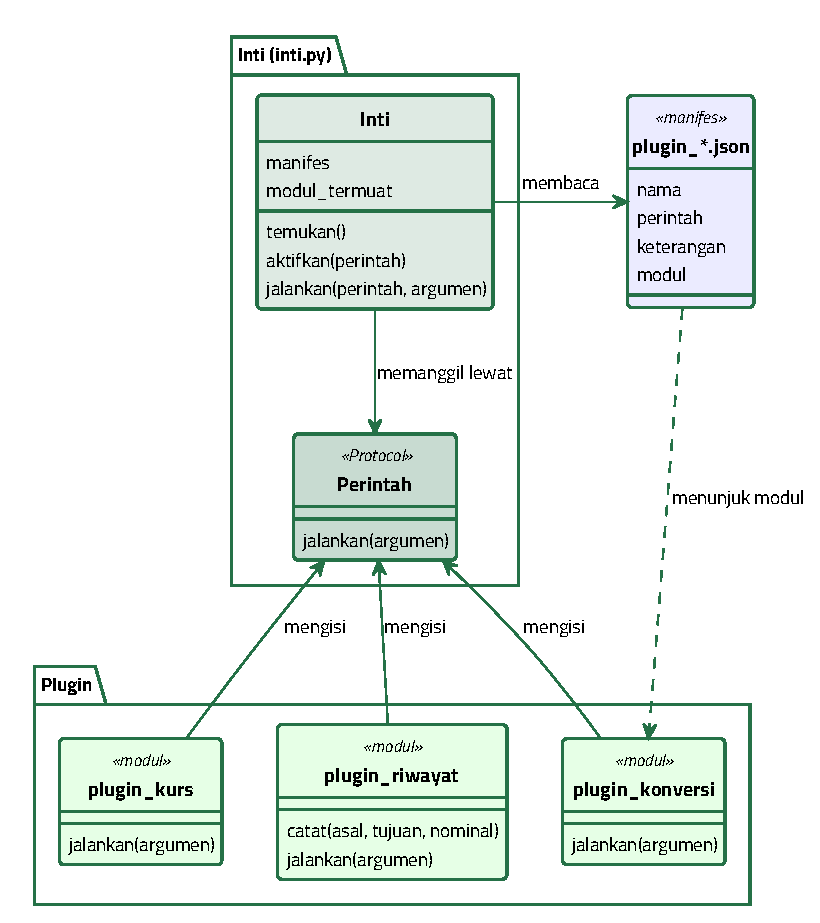
\includegraphics[width=0.78\textwidth, height=0.52\textheight,
    keepaspectratio]{kelas-microkernel.pdf}
  \caption{Inti mengenal kontrak dan manifes saja. Ketiga \textit{plugin}
    mengisi kontrak yang sama, dan manifeslah yang menunjuk nama modulnya}
  \label{fig:kelas-microkernel}
\end{figure}

\section{Kapan \textit{Plugin} Diaktifkan}

Menemukan \textit{plugin} dan mengaktifkannya adalah dua langkah yang berbeda,
dan jarak antara keduanya menentukan waktu siap sebuah aplikasi.
\textbf{Aktivasi awal} mengimpor seluruh modul saat aplikasi mulai.
\textbf{Aktivasi lambat} menunda impor sampai kemampuannya benar-benar dipakai.

Visual Studio Code memilih cara kedua. Setiap ekstensi menyatakan
\textit{activation event} pada manifesnya, misalnya \texttt{onLanguage} atau
\texttt{onCommand}, sehingga ekstensi baru dimuat ketika peristiwa itu terjadi.
Dokumentasinya bahkan menandai peristiwa yang menyala di segala keadaan sebagai
pilihan terakhir, sebab pilihan itu memperlambat awal
mula~\cite{vscode2026activation}. Eclipse menempuh jalan yang sama lewat
pemuatan yang ditunda, dan objek \textit{plugin} baru dibuat saat kemampuannya
dipakai~\cite{bolour2003eclipse}.

Mekanisme pemuatannya sudah lama dipakai di luar Python. Contoh Java pada
\berkas{sources/chapter05/java-example/} memuat setiap \textit{plugin} dari
berkas JAR tersendiri memakai \texttt{URLClassLoader}, membaca kunci
\texttt{mainclass} pada \texttt{plugin.properties}, lalu membentuk objeknya
lewat \texttt{Class.forName} beserta konstruktor hasil refleksi.
Tabel~\ref{tab:java-python} memetakan kedua sisinya.

\begin{table}[htbp]
  \centering
  \caption{Padanan mekanisme pemuatan pada contoh Java dan contoh Python}
  \label{tab:java-python}
  \begin{tabularx}{\textwidth}{|X|X|}
    \hline
    \textbf{Contoh Java} & \textbf{Contoh Python} \\
    \hline
    \texttt{plugin.properties} berisi kunci \texttt{mainclass} & \texttt{plugins/plugin\_*.json} berisi kunci \texttt{modul} dan \texttt{kelas} \\
    \hline
    \texttt{URLClassLoader} beserta \texttt{Class.forName} & \texttt{importlib.import\_module} beserta \texttt{getattr} \\
    \hline
    Konstruktor hasil refleksi menerima \texttt{Greeter} & Konstruktor kelas menerima objek \texttt{Inti} \\
    \hline
    Antarmuka \texttt{Plugin} & \textit{Protocol} \texttt{Plugin} pada \berkas{sources/chapter05/kontrak.py} \\
    \hline
  \end{tabularx}
\end{table}

Gambar~\ref{fig:sekuens-aktivasi} menunjukkan urutannya pada contoh bab ini.
Manifes dibaca saat mulai, sedangkan impor modulnya menunggu pemanggilan
pertama.

\begin{figure}[htbp]
  \centering
  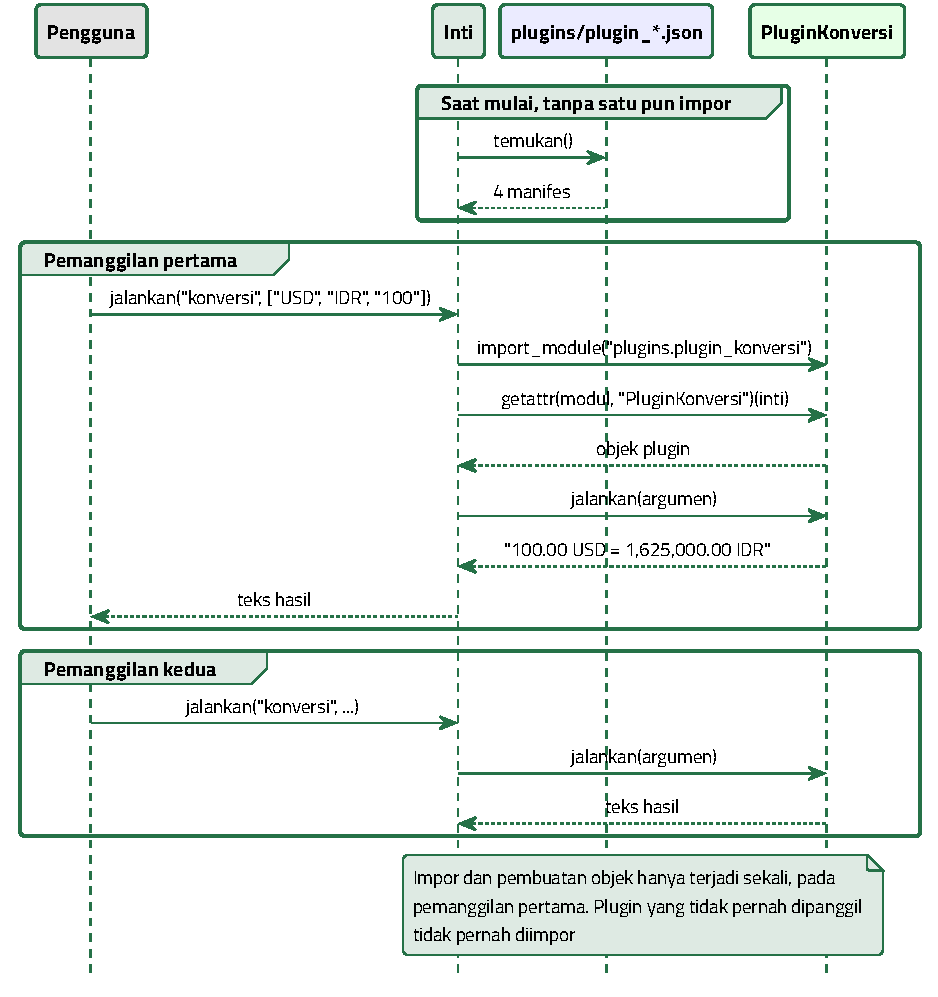
\includegraphics[width=0.95\textwidth, height=0.55\textheight,
    keepaspectratio]{sekuens-aktivasi.pdf}
  \caption{Aktivasi lambat. Impor hanya terjadi pada pemanggilan pertama, dan
    \textit{plugin} yang tidak pernah dipanggil tidak pernah diimpor}
  \label{fig:sekuens-aktivasi}
\end{figure}

Listing~\ref{lst:aktifkan} memperlihatkan intinya. Hasil impor disimpan,
sehingga pemanggilan kedua tidak membayar biaya yang sama.

\begin{lstlisting}[style=PythonStyle, caption={Aktivasi satu \textit{plugin},
  tersedia di \berkas{sources/chapter05/inti.py}}, label=lst:aktifkan]
def aktifkan(self, perintah: str) -> kontrak.Plugin:
  """Mengimpor modul, mengambil kelasnya, lalu membuat objek pluginnya."""
  if perintah in self.plugin_aktif:
    return self.plugin_aktif[perintah]  # objek pemenuh kontrak.Plugin
  manifes = self.manifes[perintah]
  try:
    modul = importlib.import_module(manifes["modul"])
    kelas = getattr(modul, manifes["kelas"])
    plugin = kelas(self)
  except Exception as kesalahan:
    self.galat_muat[perintah] = str(kesalahan)
    raise PluginGagal(f"{manifes['nama']} gagal dimuat: {kesalahan}")
  self.plugin_aktif[perintah] = plugin
  return plugin
\end{lstlisting}

\section{Ketika Satu \textit{Plugin} Rusak}

Kemampuan menerima kode dari luar membawa persoalan yang tidak dimiliki
arsitektur pada bab sebelumnya. Kode itu ditulis pihak lain, kualitasnya tidak
dapat dipastikan, dan sebagiannya pasti akan gagal. Pertanyaannya, apakah
kegagalan satu \textit{plugin} ikut menjatuhkan intinya.

Jawabannya ditentukan oleh dua keputusan. Keputusan pertama adalah kapan modul
diimpor, sebab kegagalan saat impor jauh lebih berbahaya daripada kegagalan saat
pemanggilan. Keputusan kedua adalah apakah pemanggilannya dibungkus penangkap
galat. Chrome menempuh pemisahan yang lebih jauh lagi, yaitu menjalankan
\textit{content script} di dalam \textit{isolated world} yang terpisah dari
halaman maupun dari ekstensi lain~\cite{chrome2026content}.

Kasus berikut memperlihatkan akibatnya. Sebuah tim memasang lima \textit{plugin}
pada aplikasi internalnya, dan seluruhnya diaktifkan saat aplikasi mulai. Satu
\textit{plugin} membaca berkas pengaturan pada tingkat modul, di luar fungsi
mana pun. Pada suatu pagi berkas pengaturan itu terhapus, dan impornya gagal.
Aplikasi tidak menampilkan galat satu \textit{plugin}, melainkan gagal mulai
sama sekali. Empat \textit{plugin} lain yang sehat ikut tidak berjalan, dan
pengguna tidak punya cara untuk menonaktifkan yang rusak, sebab layarnya tidak
pernah muncul.

Tabel~\ref{tab:isolasi} merangkum kedua jalur tersebut beserta akibatnya.

\begin{table}[htbp]
  \centering
  \caption{Nasib aplikasi ketika satu \textit{plugin} gagal diimpor}
  \label{tab:isolasi}
  \begin{tabularx}{\textwidth}{|l|X|X|}
    \hline
    \textbf{Jalur} & \textbf{Yang terjadi} & \textbf{Akibat bagi pengguna} \\
    \hline
    Tanpa pembungkus & Galat naik sampai ke pemanggil paling luar & Aplikasi berhenti, \textit{plugin} sehat ikut mati \\
    \hline
    Dengan pembungkus & Galat dicatat, perintah lain tetap dilayani & Satu kemampuan hilang, sisanya tetap jalan \\
    \hline
    Proses terpisah & Galat tertahan di dalam prosesnya sendiri & Aplikasi utuh, tetapi biayanya lebih mahal \\
    \hline
  \end{tabularx}
\end{table}

\section{\textit{Plugin} pada Produk Nyata}

Keempat produk berikut memakai susunan yang sama dengan nama yang berbeda.
Tabel~\ref{tab:produk-plugin} merangkum istilah dan berkas manifes masing-masing.

\begin{table}[htbp]
  \centering
  \caption{Sebutan dan berkas manifes pada empat produk yang memakai
    \textit{plugin}}
  \label{tab:produk-plugin}
  \begin{tabularx}{\textwidth}{|l|l|X|}
    \hline
    \textbf{Produk} & \textbf{Manifes} & \textbf{Catatan} \\
    \hline
    Eclipse & \texttt{plugin.xml} & Kontraknya disebut \textit{extension point}, dan pengisinya disebut \textit{extension} \\
    \hline
    Visual Studio Code & \texttt{package.json} & Pemuatan ditunda sampai \textit{activation event} yang didaftarkan terjadi \\
    \hline
    Chrome & \texttt{manifest.json} & \textit{Content script} berjalan di \textit{isolated world} yang terpisah \\
    \hline
    Firefox & \texttt{manifest.json} & Memakai model WebExtensions yang sama, dengan sejumlah perbedaan yang disengaja \\
    \hline
  \end{tabularx}
\end{table}

Perbedaan namanya menutupi kesamaan susunannya. Ketiganya menyimpan manifes di
luar kode, menunda pemuatan, dan menolak menyebut nama penyumbang di dalam
intinya. Yang berbeda hanyalah seberapa jauh pemisahannya dibawa, dan Chrome
membawanya paling jauh dengan memisahkan lingkungan eksekusinya.

\section{Ringkasan}

Microkernel membagi sistem menjadi inti yang kecil beserta bagian tambahan yang
dapat dipasang dan dicabut. Bentuk yang paling sering ditemui bukan kernel
sistem operasi, melainkan arsitektur \textit{plugin} pada perkakas sehari-hari.
Eclipse, Visual Studio Code, Chrome, dan Firefox sama-sama memakainya.

Yang membuat susunan tersebut bekerja adalah arah pengenalan. Inti menulis
kontrak dan membaca manifes, sedangkan \textit{plugin} yang mengisi kontrak
tersebut. Karena inti tidak pernah menyebut nama satu penyumbang pun, menambah
kemampuan berarti menambah berkas, bukan menyunting inti. Latihan~1 membuktikan
klaim itu dengan menghitung penyebutannya, dan angkanya nol.

Manifes yang terpisah dari kode membuka pilihan kedua, yaitu kapan sebuah
\textit{plugin} diaktifkan. Aktivasi lambat membaca manifes saat mulai lalu
menunda impor sampai kemampuannya dipakai. Pada contoh bab ini, cara tersebut
membuat waktu siap 3,3 kali lebih cepat, dan selisihnya lebih besar daripada
\textit{range} pengukurannya sendiri. Kesimpulan itu berbeda dengan Bab~2, dan
perbedaannya justru memperlihatkan gunanya membandingkan selisih dengan
\textit{range}.

Kemampuan menerima kode dari luar menuntut harga tersendiri. Satu
\textit{plugin} yang gagal saat impor dapat menjatuhkan seluruh aplikasi bila
pemanggilannya tidak dibungkus. Latihan~2 memperlihatkan selisihnya, yaitu tiga
perintah tetap berjalan pada jalur berpelindung, sedangkan jalur tanpa
pelindung berhenti pada berkas yang rusak.

Pesan utama bab ini karena itu bukan bahwa inti harus kecil, melainkan bahwa
inti harus buta terhadap penyumbangnya. Kebutaan itu yang dibayar dengan
kontrak, manifes, dan registri, dan ketiganya baru terasa mahal ketika jumlah
\textit{plugin} masih sedikit.

\section{Latihan}

Ketiga latihan berikut memakai satu basis kode yang sama di
\berkas{sources/chapter05/}, tetapi menyasar tiga masalah yang berbeda.
Latihan~1 memeriksa penyebutan \textit{plugin} di dalam inti. Latihan~2
memeriksa akibat satu \textit{plugin} yang rusak. Latihan~3 mengukur selisih
waktu siap antara kedua cara aktivasi. Hasil setiap mahasiswa dapat berbeda,
dan yang dilaporkan adalah pola perbandingannya, bukan angka mutlaknya.

Venv yang sama dipakai kembali, dan pengaktifannya seperti pada
Listing~\ref{lst:venv-ch05}. Latihan bab ini hanya memakai pustaka standar
Python, sehingga tidak ada pemasangan tambahan.

\begin{lstlisting}[language=bash, caption={Mengaktifkan venv sebelum ketiga
  latihan, skrip tersedia di \berkas{sources/siapkan_venv.sh}},
  label=lst:venv-ch05]
bash sources/siapkan_venv.sh
source .venv/bin/activate
cd sources/chapter05
python inti.py daftar
# Keluarannya baris pertama: Plugin terpasang: 4
\end{lstlisting}

\subsection*{Latihan 1: Menghitung Penyebutan \textit{Plugin} di Dalam Inti}

Latihan ini menguji klaim utama arsitektur \textit{plugin}, yaitu menambah
kemampuan cukup dengan menambah berkas. Klaim tersebut menyebut angka, sehingga
dapat dibuktikan salah. Satu penyebutan nama modul \textit{plugin} di dalam inti
sudah cukup untuk menggugurkannya. Langkah kerjanya sebagai berikut.

\begin{enumerate}
  \item Jalankan \texttt{python periksa\_inti.py}, lalu catat baris
    \texttt{Plugin disebut inti} beserta ketiga angka di bawahnya.
  \item Buka \berkas{sources/chapter05/inti.py}, lalu cari nama modul
    \textit{plugin} di dalamnya. Catat hasil pencarian itu.
  \item Salin \berkas{sources/chapter05/plugins/plugin_riwayat.py} beserta
    manifesnya menjadi \texttt{plugin\_pajak.py}, lalu ubah nama, perintah, dan
    nama kelasnya.
  \item Jalankan \texttt{python inti.py daftar}, lalu catat jumlah
    \textit{plugin} yang terbaca.
  \item Jalankan ulang \texttt{python periksa\_inti.py}, lalu catat berapa baris
    inti yang berubah selama langkah ketiga dan keempat.
\end{enumerate}

Tabel~\ref{tab:lat1plugin-contoh} berisi hasil satu kali pemeriksaan nyata.

\begin{table}[htbp]
  \centering
  \caption{Contoh hasil Latihan 1 yang sudah terisi}
  \label{tab:lat1plugin-contoh}
  \begin{tabularx}{\textwidth}{|X|l|}
    \hline
    \textbf{Yang dilaporkan} & \textbf{Nilai} \\
    \hline
    Manifes ditemukan & 4 \\
    \hline
    \textit{Plugin} disebut inti & 0 \\
    \hline
    Baris inti & 128 \\
    \hline
    Baris seluruh \textit{plugin} & 104 \\
    \hline
    Bagian \textit{plugin} & 45 persen \\
    \hline
  \end{tabularx}
\end{table}

Isikan hasil pemeriksaan pada Tabel~\ref{tab:lat1plugin-hasil}.

\begin{table}[htbp]
  \centering
  \caption{Lembar isian Latihan 1}
  \label{tab:lat1plugin-hasil}
  \begin{tabularx}{\textwidth}{|X|l|l|}
    \hline
    \textbf{Yang dilaporkan} & \textbf{Sebelum} & \textbf{Sesudah} \\
    \hline
    Manifes ditemukan & \dots & \dots \\
    \hline
    \textit{Plugin} disebut inti & \dots & \dots \\
    \hline
    Baris inti & \dots & \dots \\
    \hline
    Baris seluruh \textit{plugin} & \dots & \dots \\
    \hline
  \end{tabularx}
\end{table}

Jawab tiga pertanyaan berikut dengan menunjuk angka pada tabel. Pertama, baris
inti tidak berubah sama sekali walaupun satu \textit{plugin} ditambahkan.
Sebutkan bagian inti yang membuat hal itu mungkin. Kedua, jelaskan apa yang akan
terjadi pada angka penyebutan bila inti mengimpor satu \textit{plugin} secara
langsung demi kemudahan. Ketiga, hitung bagian kode yang berupa \textit{plugin},
lalu bandingkan dengan perkiraan awal sebelum pengukuran dilakukan.

\subsection*{Latihan 2: Menjatuhkan Aplikasi dengan Satu \textit{Plugin}}

Latihan ini membuktikan bahwa kegagalan satu \textit{plugin} tidak harus
menjatuhkan intinya. Berkas \berkas{sources/chapter05/plugin_rusak.py} sengaja
gagal pada tingkat modul, sehingga kegagalannya muncul saat impor. Langkah
kerjanya sebagai berikut.

\begin{enumerate}
  \item Baca \berkas{sources/chapter05/plugins/plugin_rusak.py}, lalu
    tunjukkan baris yang menyebabkan kegagalannya.
  \item Jalankan \texttt{python uji\_isolasi.py}, lalu catat kedua baris
    hasilnya.
  \item Jalankan \texttt{python inti.py rusak} dan \texttt{python inti.py kurs}
    berurutan, lalu catat apakah perintah kedua tetap dilayani.
  \item Buka \berkas{sources/chapter05/inti.py}, lalu temukan bagian yang
    membungkus galat impor.
  \item Hapus sementara pembungkus tersebut, jalankan ulang
    \texttt{python inti.py kurs}, lalu catat akibatnya. Kembalikan kodenya
    sesudah dicatat.
\end{enumerate}

Tabel~\ref{tab:lat2plugin-contoh} berisi hasil satu kali percobaan nyata.

\begin{table}[htbp]
  \centering
  \caption{Contoh hasil Latihan 2 yang sudah terisi}
  \label{tab:lat2plugin-contoh}
  \begin{tabularx}{\textwidth}{|l|l|X|}
    \hline
    \textbf{Jalur} & \textbf{Perintah jalan} & \textbf{Catatan} \\
    \hline
    Dengan pelindung & 3 dari 4 & Satu \textit{plugin} dilewati, sisanya dilayani \\
    \hline
    Tanpa pelindung & 3 modul & Berhenti pada \texttt{plugin\_rusak} \\
    \hline
  \end{tabularx}
\end{table}

Isikan hasil percobaan pada Tabel~\ref{tab:lat2plugin-hasil}.

\begin{table}[htbp]
  \centering
  \caption{Lembar isian Latihan 2}
  \label{tab:lat2plugin-hasil}
  \begin{tabularx}{\textwidth}{|l|l|X|}
    \hline
    \textbf{Jalur} & \textbf{Perintah jalan} & \textbf{Catatan} \\
    \hline
    Dengan pelindung & \dots & \dots \\
    \hline
    Tanpa pelindung & \dots & \dots \\
    \hline
    Tanpa pembungkus galat & \dots & \dots \\
    \hline
  \end{tabularx}
\end{table}

Jawab tiga pertanyaan berikut. Pertama, jelaskan mengapa kegagalan saat impor
lebih berbahaya daripada kegagalan saat pemanggilan. Kedua, sebutkan apa yang
hilang bagi pengguna ketika satu \textit{plugin} dilewati, lalu bandingkan
dengan yang hilang ketika aplikasi tidak mau mulai. Ketiga, jelaskan mengapa
pemisahan proses seperti pada Chrome lebih kuat daripada pembungkus galat,
beserta harga yang dibayarnya.

\subsection*{Latihan 3: Mengukur Biaya Aktivasi Awal}

Latihan ini mengukur selisih waktu siap antara aktivasi lambat dan aktivasi
awal. Pengukurannya diulang seratus putaran, sebab satu putaran tidak cukup
untuk menyimpulkan apa pun. Cache impor Python dibersihkan pada setiap putaran,
agar kedua jalur menghadapi keadaan yang sama. Langkah kerjanya sebagai berikut.

\begin{enumerate}
  \item Jalankan \texttt{python ukur\_aktivasi.py}. Skrip tersebut mencetak
    baris kemajuan setiap sepuluh putaran, sehingga jalannya terlihat.
  \item Catat kedelapan angka pada laporan akhirnya.
  \item Buka \berkas{sources/chapter05/ukur_aktivasi.py}, lalu tunjukkan baris
    yang membersihkan cache impor.
  \item Hapus sementara pembersihan tersebut, jalankan ulang, lalu catat
    perubahan angkanya. Kembalikan kodenya sesudah dicatat.
\end{enumerate}

Tabel~\ref{tab:lat3plugin-contoh} berisi hasil satu kali pengukuran nyata.

\begin{table}[htbp]
  \centering
  \caption{Contoh hasil Latihan 3 yang sudah terisi, seratus putaran}
  \label{tab:lat3plugin-contoh}
  \begin{tabularx}{\textwidth}{|X|l|}
    \hline
    \textbf{Yang dilaporkan} & \textbf{Nilai} \\
    \hline
    Median aktivasi lambat & 0,4006 ms \\
    \hline
    Median aktivasi awal & 1,3406 ms \\
    \hline
    Selisih median antar jalur & 0,9399 ms \\
    \hline
    Aktivasi awal lebih lambat & 3,3 kali \\
    \hline
    \textit{Range} di dalam jalur lambat & 0,2896 ms \\
    \hline
    \textit{Range} dibagi selisih & 0,3 kali \\
    \hline
    Putaran lambat lebih cepat & 100 dari 100 \\
    \hline
  \end{tabularx}
\end{table}

Baris keenam itulah yang membedakan bab ini dari Bab~2. Di sana \textit{range}
di dalam satu jalur puluhan kali lebih besar daripada selisih yang dicari,
sehingga selisihnya belum dapat disebut ada. Di sini \textit{range}-nya justru
sepertiga selisihnya, dan pencacahan per putaran menegaskannya dengan angka
100 dari 100. Selisih yang seperti inilah yang layak dilaporkan.

Isikan hasil pengukuran pada Tabel~\ref{tab:lat3plugin-hasil}.

\begin{table}[htbp]
  \centering
  \caption{Lembar isian Latihan 3}
  \label{tab:lat3plugin-hasil}
  \begin{tabularx}{\textwidth}{|X|l|l|}
    \hline
    \textbf{Yang dilaporkan} & \textbf{Dengan pembersihan} & \textbf{Tanpa pembersihan} \\
    \hline
    Median aktivasi lambat & \dots & \dots \\
    \hline
    Median aktivasi awal & \dots & \dots \\
    \hline
    Selisih median antar jalur & \dots & \dots \\
    \hline
    \textit{Range} dibagi selisih & \dots & \dots \\
    \hline
    Putaran lambat lebih cepat & \dots & \dots \\
    \hline
  \end{tabularx}
\end{table}

Jawab tiga pertanyaan berikut dengan menunjuk angka pada tabel. Pertama,
jelaskan mengapa selisih pada bab ini layak disebut ada, sedangkan selisih pada
Bab~2 tidak. Kedua, jelaskan apa yang terjadi pada angka ketika pembersihan
cache dihapus, lalu sebutkan pengukuran mana yang menjadi tidak jujur karenanya.
Ketiga, dengan menggabungkan hasil ketiga latihan, tentukan kapan aktivasi awal
tetap layak dipilih walaupun lebih lambat, lalu sebutkan angka yang menjadi
dasar keputusannya.

  %\include{chapter06}
  %\include{chapter07}
  %\include{chapter08}
  %\include{chapter09}
  %\include{chapter10}
  %\include{chapter11}
  %\include{chapter12}
  %\include{chapter13}
  %\include{chapter14}
  %\appendix
  %\include{appendixA}
  %\include{appendixB}

  \backmatter
  \addcontentsline{toc}{chapter}{Daftar Pustaka}
  \bibliographystyle{plainnat}
  \bibliography{references}

\end{document}
